\documentclass[table]{beamer}
%[]中可以使用draft、handout、screen、transparency、trancompress、compress等参数

%指定beamer的模式与主题
\mode<presentation>
{
  \usetheme{Madrid}
%\usetheme{Boadilla}
%\usecolortheme{default}
%\usecolortheme{orchid}
%\usecolortheme{whale}
%\usefonttheme{professionalfonts}
}

%\usetheme{Madrid}
%这里还可以选择别的主题:Bergen, Boadilla, Madrid, AnnArbor, CambridgeUS, Pittsburgh, Rochester, Warsaw, ...
%有导航栏的Antibes, JuanLesPins, Montpellier, ...
%有内容的Berkeley, PaloAlto, Goettingen, Marburg, Hannover, ...
%有最小导航栏的Berlin, Ilmenau, Dresden, Darmstadt, Frankfurt, Singapore, Szeged, ...
%有章和节表单的Copenhagen, Luebeck, Malmoe, Warsaw, ...

%\usecolortheme{default}
%设置内部颜色主题(这些主题一般改变block里的颜色);这个主题一般选择动物来命名
%这里还可以选择别的颜色主题,如默认的和有特别目的的颜色主题default,structure,sidebartab,全颜色主题albatross,beetle,crane,dove,fly,seagull,wolverine,beaver

%\usecolortheme{orchid}
%设置外部颜色主题(这些主题一般改变title里的颜色);这个主题一般选择植物来命名
%这里还可以选择别的颜色主题,如默认的和有特别目的的颜色主题lily,orchid,rose

%\usecolortheme{whale}
%设置字体主题;这个主题一般选择海洋动物来命名
%这里还可以选择别的颜色主题,如默认的和有特别目的的颜色主题whale,seahorse,dolphin

%\usefonttheme{professionalfonts}
%类似的还可以定义structurebold,structuresmallcapsserif,professionalfonts

% 控制 beamer 的风格,可以根据自己的爱好修改
%\usepackage{beamerthemesplit} %使用 split 风格
%\usepackage{beamerthemeshadow} %使用 shadow 风格
%\usepackage[width=2cm,dark,tab]{beamerthemesidebar}

%插入音标
%\usepackage{tipa}
%\AtBeginDocument{
  %\renewcommand\textipa{\fontencoding{T3}\selectfont}
%}
%\AtBeginDocument{
  %\renewcommand\textipa[2][r]{{\fontfamily{cm#1}\tipaencoding #2}}
%}
%\renewenvironment{IPA}[1][r]
 %{\fontfamily{cm#1}\tipaencoding}
 %{}

% 设定英文字体
%\usepackage{fontspec}
% Fix bugs for fontspec in TeXLive2015
\ifdefined\suppressfontnotfounderror
  \expandafter\let\csname xetex_suppressfontnotfounderror:D\endcsname
    \suppressfontnotfounderror
\else
  \expandafter\let\csname xetex_suppressfontnotfounderror:D\endcsname
    \luatexsuppressfontnotfounderror
\fi
\usepackage[no-math]{fontspec}
\setmainfont{Times New Roman}
\setsansfont{Arial}
\setmonofont{Courier New}

% 设定中文字体
\usepackage[BoldFont,SlantFont,CJKchecksingle,CJKnumber]{xeCJK}
%\setCJKmainfont[BoldFont={Adobe Heiti Std},ItalicFont={Adobe Kaiti Std}]{Adobe Song Std}
\setCJKmainfont[BoldFont={Adobe Heiti Std},ItalicFont={Adobe Kaiti Std}]{WenQuanYi Micro Hei}
\setCJKsansfont{Adobe Heiti Std}
\setCJKmonofont{Adobe Fangsong Std}
\punctstyle{hangmobanjiao}

\defaultfontfeatures{Mapping=tex-text}
\usepackage{xunicode}
\usepackage{xltxtra}

\XeTeXlinebreaklocale "zh"
\XeTeXlinebreakskip = 0pt plus 1pt minus 0.1pt

\usepackage{setspace}
\usepackage{colortbl,xcolor}
\usepackage{hyperref}
%\hypersetup{xetex,bookmarksnumbered=true,bookmarksopen=true,pdfborder=1,breaklinks,colorlinks,linkcolor=blue,filecolor=black,urlcolor=cyan,citecolor=green}
\hypersetup{xetex,bookmarksnumbered=true,bookmarksopen=true,pdfborder=1,breaklinks,colorlinks,linkcolor=cyan,filecolor=black,urlcolor=blue,citecolor=green}

% 插入图片
\usepackage{graphicx}
\graphicspath{{figures/}}
% 图文混排
%\usepackage{picins}
\usepackage{floatflt}

% 可能用到的包
\usepackage{amsmath,amssymb}
%插入多媒体
%\usepackage{media9}
%\usepackage{movie15}
\usepackage{multimedia}
\usepackage{multicol}
\usepackage{multirow}

% 定义一些自选的模板,包括背景、图标、导航条和页脚等,修改要慎重
% 设置背景渐变由10%的红变成10%的结构颜色
%\beamertemplateshadingbackground{red!10}{structure!10}
%\beamertemplatesolidbackgroundcolor{white!90!blue}
% 使所有隐藏的文本完全透明、动态,而且动态的范围很小
\beamertemplatetransparentcovereddynamic
% 使itemize环境中变成小球,这是一种视觉效果
\beamertemplateballitem
% 为所有已编号的部分设置一个章节目录,并且编号显示成小球
\beamertemplatenumberedballsectiontoc
% 将每一页的要素的要素名设成加粗字体
\beamertemplateboldpartpage

% item逐步显示时,使已经出现的item、正在显示的item、将要出现的item呈现不同颜色
\def\hilite<#1>{
 \temporal<#1>{\color{gray}}{\color{blue}}
    {\color{blue!25}}
}

\renewcommand{\today}{\number\year 年 \number\month 月 \number\day 日}

%五角星
\usepackage{MnSymbol}

%去除图表标题中的figure等
\usepackage{caption}
\captionsetup{labelformat=empty,labelsep=none}

\usepackage{tabu}
\usepackage{multirow}
%表格自动换行
\usepackage{tabularx} 

% 千分号
%\usepackage{textcomp}

%罗马数字
\makeatletter
\newcommand{\rmnum}[1]{\romannumeral #1}
\newcommand{\Rmnum}[1]{\expandafter\@slowromancap\romannumeral #1@}
\makeatother

%分栏
\usepackage{multicol}

%\usepackage{enumitem}
%\usepackage{enumerate}

%键盘
\usepackage{keystroke}

%心形
\usepackage{fdsymbol}

%插入源代码
\usepackage{listings}
\lstset{
  language=perl,                  % 程序语言名称:TeX, Perl, R, sh, bash, Awk
  basicstyle=\normalsize\tt,      %\tt指monospace字体族,程序源代码使用此族字体表示更加美观
  numbers=left,                   % 行号位置(左侧)
  numberstyle=\small,             % 行号字体的字号
  stepnumber=1,                   % 行号的显示步长
  numbersep=5pt,                  % 行号与代码间距
  backgroundcolor=\color{white},  % 背景色;需要 \usepackage{color}
  showspaces=false,               % 不显示空格
  showstringspaces=false,         % 不显示代码字符串中的空格标记
  showtabs=false,                 % 不显示 TAB
  tabsize=4, 
  frame=shadowbox,                % 把代码用带有阴影的框圈起来
  captionpos=b,                   % 标题位置
  breaklines=true,                % 对过长的代码自动断行
  breakatwhitespace=false,        % 断行只在空格处
  extendedchars=false,            % 解决代码跨页时,章节标题,页眉等汉字不显示的问题
  %escapeinside={\%*}{*},         % 跳脱字符,添加注释,暂时离开 listings 
  %escapeinside=``,
  commentstyle=\color{red!50!green!50!blue!50}\tt,  %浅灰色的注释
  rulesepcolor=\color{red!20!green!20!blue!20},     %代码块边框为淡青色
  keywordstyle=\color{blue!70}\bfseries\tt,         %代码关键字的颜色为蓝色,粗体
  identifierstyle=\tt,
  stringstyle=\tt,                % 代码字符串的特殊格式
  keepspaces=true,
  breakindent=1em,
  %breakindent=22pt,
  %breakindent=4em,
  breakautoindent=true,
  flexiblecolumns=true,
  aboveskip=1em,                  %代码块边框
  xleftmargin=2em,
  xrightmargin=2em
}

%\setbeamercolor{alerted text}{fg=magenta}
\setbeamercolor{bgcolor}{fg=yellow,bg=cyan}
%\setbeamercolor{itemize/enumerate body}{fg=green}

\begin{document}

%\includeonlyframes{current}

\logo{\includegraphics[height=0.08\textwidth]{tijmu.png}}

% 在每个Section前都会加入的Frame
\AtBeginSection[]
{
  \begin{frame}<beamer>
    %\frametitle{Outline}
    \frametitle{教学提纲}
    \setcounter{tocdepth}{3}
    \begin{multicols}{2}
      \tableofcontents[currentsection,currentsubsection]
      %\tableofcontents[currentsection]
    \end{multicols}
  \end{frame}
}
% 在每个Subsection前都会加入的Frame
\AtBeginSubsection[]
{
  \begin{frame}<beamer>
%%\begin{frame}<handout:0>
%% handout:0 表示只在手稿中出现
    \frametitle{教学提纲}
    \setcounter{tocdepth}{3}
    \begin{multicols}{2}
    \tableofcontents[currentsection,currentsubsection]
    \end{multicols}
%% 显示在目录中加亮的当前章节
  \end{frame}
}

% 为当前幻灯片设置背景
%{
%\usebackgroundtemplate{
%\vbox to \paperheight{\vfil\hbox to
%\paperwidth{\hfil\includegraphics[width=2in]{tijmu_charcoal.png}\hfil}\vfil}
%}
\begin{frame}[plain]
  \begin{center}
    {\Huge 分子生物计算\\}
    {\huge \textit{(Perl语言编程)}\\}
    \vspace{1cm}
    {\LARGE 天津医科大学\\}
    %\vspace{0.2cm}
    {\LARGE 生物医学工程与技术学院\\}
    \vspace{1cm}
    {\large 2019-2020学年上学期(秋)\\ 2017级生信班}
  \end{center}
\end{frame}
%}



%\includeonlyframes{current}

\title[Perl语言入门]{第二章\quad Perl语言入门}
\author[Yixf]{伊现富(Yi Xianfu)}
\institute[TIJMU]{天津医科大学(TIJMU)\\ 生物医学工程与技术学院}
\date{2019年9月}

\input{snippet/beamer_toc.tex}

\section{引言}
\begin{frame}
  \frametitle{引言 | 计算机}
  \begin{figure}
    \centering
    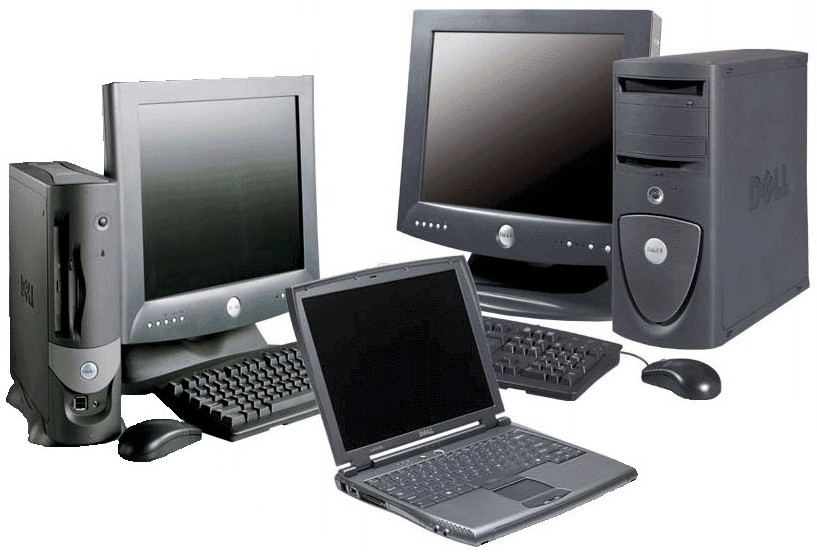
\includegraphics[width=10cm]{c2_perl_computer_01.jpg}
  \end{figure}
\end{frame}

\begin{frame}
  \frametitle{引言 | 计算机程序}
  计算机程序(computer program)是指一组指示计算机或其他具有信息处理能力装置每一步动作的\alert{指令},通常用某种程序设计语言编写,运行于某种目标体系结构上。\\
  \vspace{1em}
  打个比方,一个程序就像一个用汉语(程序设计语言)写下的红烧肉菜谱(程序),用于指导懂汉语和烹饪手法的人(体系结构)来做这个菜。\\
  \vspace{1em}
  通常,计算机程序要经过编译和链接而成为一种人们不易看懂而计算机可解读的格式,然后运行。未经编译就可运行的程序,通常称之为\alert{脚本}程序(script)。
\end{frame}

\begin{frame}
  \frametitle{引言 | 编程语言}
编程语言(programming language),是用来定义计算机程序的形式语言。它是一种被标准化的交流技巧,用来向计算机发出指令。一种计算机语言让程序员能够准确地定义计算机所需要使用的数据,并精确地定义在不同情况下所应当采取的行动。\\
  \vspace{1em}
  与英语类似,编程语言其实就是一门\alert{外语},只不过是专门用于跟计算机进行沟通的外语。\\
  \vspace{1em}
在电脑领域已发明了上千种不同的编程语言,而且每年仍有新的编程语言诞生。有许多用于特殊用途的语言,只在特殊情况下使用。例如,PHP专门用来显示网页;Perl更适合文本处理;C语言被广泛用于操作系统和编译器的开发(所谓的系统编程)。
\end{frame}

\section{Perl简介}
\begin{frame}
  \frametitle{Perl | 简介}
  \begin{block}{Perl}
    \begin{itemize}
      \item Perl是高级、通用、直译式、动态的程序语言
      \item \alert{Practical Extraction and Report Language},实用摘录与报表语言
      \item Pathologically Eclectic Rubbish Lister,病态折中式垃圾列表器
      \item 拉里·沃尔(\alert{Larry Wall}),\alert{1987年} 12月18日
    \end{itemize}
  \end{block}
  \pause
  \begin{block}{特性}
    \begin{itemize}
      \item 具有动态语言强大灵活的特性
      \item 借用了C、sed、AWK、shell等语言的特性,提供了许多冗余语法
      \item 使用了语言学的思维(泛型变量、动态数组、Hash表等)
      \item 程序员可以忽略内部数据存储、类型、内存越界等细节
      \item 内部集成了正则表达式的功能
      \item 巨大的第三方代码库 \alert{CPAN}(\href{http://www.cpan.org/}{Comprehensive Perl Archive Network},Perl综合典藏网);搜索引擎 \href{https://metacpan.org/}{MetaCPAN}
    \end{itemize}
  \end{block}
\end{frame}

\begin{frame}
  \frametitle{Perl | 简介 | Larry Wall}
  \begin{block}{简介}
    1954年,程序员、系统管理员、语言学家和作家。
  \end{block}
  \pause
  \begin{block}{在Perl里的工作(来自Perl官方文档)}
    \begin{itemize}
      \item 拉里对Perl如何表现的定义总是对的。这说明他对核心功能有最终否决权。
      \item 拉里可以日后改变对任何东西的看法,不论他以前是否使用了规则1。(拉里总是对的,即使当他原来是错的。)
      %\item (懂了么?拉里总是对的,即使他原来是错的。)
    \end{itemize}
  \end{block}
  \pause
  \begin{block}{程序员的3个美德}
    \begin{itemize}
      %\item 懒惰:这个品质使你尽最大的努力去减少总的精力消耗。这让你写出节省劳动力的程序,而且别人会找到有用的地方,和你写的文档。所以你不需要回答关于该软件的很多问题。因此是程序员的第一个美德。参见不耐烦和骄傲。
      %\item 不耐烦:当电脑懒惰的时候你感觉生气。这让你写出不仅反映你的需求,而实际上预先使用它们。或者至少假装。所以是程序员的第二个美德。参见懒惰和骄傲。
      %\item 骄傲:极度骄傲,宙斯快速推动你想要的那种东西。同时这个品质让你写(和维护)别人支持的程序。所以是程序员的第三个美德。参见懒惰和不耐烦。
      \item 懒惰(Laziness);不耐烦(Impatience);骄傲(Hubris)
      \item (出处:《Programming Perl》(《骆驼书》)第二版,沃尔(和共同作者Randal L.  Schwartz与Tom Christiansen)
    \end{itemize}
  \end{block}
\end{frame}

\begin{frame}
  \frametitle{Perl | 简介 | “三美”程序员}
  \vspace{-0.5em}
  \begin{block}{懒惰(Laziness)}
 {\footnotesize   是这样一种品质,它使得你花大力气去避免消耗过多的精力。它敦促你写出节省体力的程序,同时别人也能利用它们。为此你会写出完善的文档,以免别人问你太多问题。\\
 The quality that makes you go to great effort to reduce overall energy expenditure. It makes you write labor-saving programs that other people will find useful, and document what you wrote so you don't have to answer so many questions about it.}
  \end{block}
  \vspace{-0.5em}
  \begin{block}{急躁(Impatience)}
{\footnotesize
    是这样一种愤怒——当你发现计算机懒洋洋地不给出结果。于是你写出更优秀的代码,能尽快真正的解决问题。至少看上去是这样。\\
    The anger you feel when the computer is being lazy. This makes you write programs that don't just react to your needs, but actually anticipate them. Or at least pretend to.}
  \end{block}
  \vspace{-0.5em}
  \begin{block}{傲慢(Hubris)}
{\footnotesize
    极度的自信,使你有信心写出(或维护)别人挑不出毛病的程序。\\
    Excessive pride, the sort of thing Zeus zaps you for. Also the quality that makes you write (and maintain) programs that other people won't want to say bad things about.}
  \end{block}
\end{frame}

\begin{frame}
  \frametitle{Perl | 简介}
  \begin{block}{\alert{书写规范}}
    \begin{itemize}
      \item Perl:程序语言本身
      \item perl:实际编译并运行程序的解释器
      \item PERL:错误的写法(外行的标志)
    \end{itemize}
  \end{block}
\end{frame}

\begin{frame}
  \frametitle{Perl | 应用}
  \begin{block}{应用}
    Perl擅长处理整体来说“约有90\%与文字处理有关,10\%与其他事物有关”的问题。 
  \end{block}
  \begin{block}{领域}
    \begin{itemize}
      \item 网络编程、CGI(Common Gateway Interface,通用网关接口)
      \item 图形编程
      \item 系统管理
      \item 生物信息
      \item \ldots
    \end{itemize}
  \end{block}
\end{frame}

\begin{frame}
  \frametitle{Perl | 应用}
  \begin{block}{名号}
    \begin{itemize}
      \item 脚本语言中的瑞士军刀
      \item Unix中的王牌工具
      \item 一种拥有各种语言功能的梦幻脚本语言
      \item 名符其实的“胶水语言”
      \item 黑客语言
      \item 拯救人类基因组计划的“利器”
      \item 与Python并称为生物信息学家的语言
      \item \ldots
    \end{itemize}
  \end{block}
\end{frame}

\begin{frame}
  \frametitle{Perl | 应用}
  \begin{block}{应用举例}
    \begin{description}
      \item[\alert{Asciiquarium}] Asciiquarium is an aquarium/sea animation in ASCII art. Enjoy the mysteries of the sea from the safety of your own terminal! 
      \item[\alert{ack}] ack is a code-searching tool, similar to grep but optimized for programmers searching large trees of source code. It runs in pure Perl, is highly portable, and runs on any platform that runs Perl. 
      \item[Mojo-Webqq] 使用Perl语言编写的smartqq/webqq客户端框架(非GUI)。 
      \item[Mojo-Weixin] 使用Perl语言编写的微信/weixin/wechat客户端框架(非GUI)。
    \end{description}
  \end{block}
\end{frame}

\begin{frame}
  \frametitle{Perl | 应用}
  {\footnotesize
    \begin{block}{应用举例}
    \begin{description}
      \item[\alert{Bugzilla}] Bugzilla is free and open source web-based bug-tracking software that is developed by an active group of volunteers in the Mozilla community, and used by thousands of projects and companies around the world. 
      \item[RT] RT is an enterprise-grade issue tracking system. It allows organizations to keep track of what needs to get done, who is working on which tasks, what's already been done, and when tasks were (or weren't) completed.
      \item[\alert{Webmin}] Webmin is a web-based interface for system administration for Unix. Using any browser that supports tables and forms, you can setup user accounts, Apache, internet services, DNS, file sharing and so on.
      \item[\alert{Circos}] Circos is a program for the generation of publication-quality, circularly composited renditions of genomic data and related annotations. Circos is particularly suited for visualizing alignments, conservation and intra and inter-chromosomal relationships.
    \end{description}
  \end{block}
  }
\end{frame}

\begin{frame}
  \frametitle{Perl | 应用}
  {\footnotesize
    \begin{block}{应用举例}
    \begin{description}
      \item[Frozen Bubble] Frozen Bubble是一款泡泡龙样式的可在多个操作系统上运行的自由软体电脑游戏。Frozen Bubble原版用 Perl写成,拥有100个关卡,附带关卡编辑器。和很多专门针对Linux开发的游戏一样,使用Tux为主要角色,发射彩色冰泡泡到同色的泡泡旁边,成组消灭它们。在泡泡到达底部之前全部消除。 
      \item[Movable Type] Movable Type,简称MT,是由位于美国加州的Six Apart公司推出的博客发布系统。它是全球最受欢迎的博客系统之一,包含多用户、评论、引用、主题等功能,并广泛的支持各种第三方插件。Movable Type不仅可以应用于个人的博客系统,而且可以应用于商业、教育等领域。 
      \item[TWiki] TWiki is a Perl-based structured wiki application, typically used to run a collaboration platform, knowledge or document management system, a knowledge base, or team portal. Users can create wiki pages using the TWiki Markup Language, and developers can extend wiki application functionality with plugins.
    \end{description}
  \end{block}
  }
\end{frame}

\begin{frame}
  \frametitle{Perl | 应用 | Asciiquarium}
  \begin{figure}
    \centering
    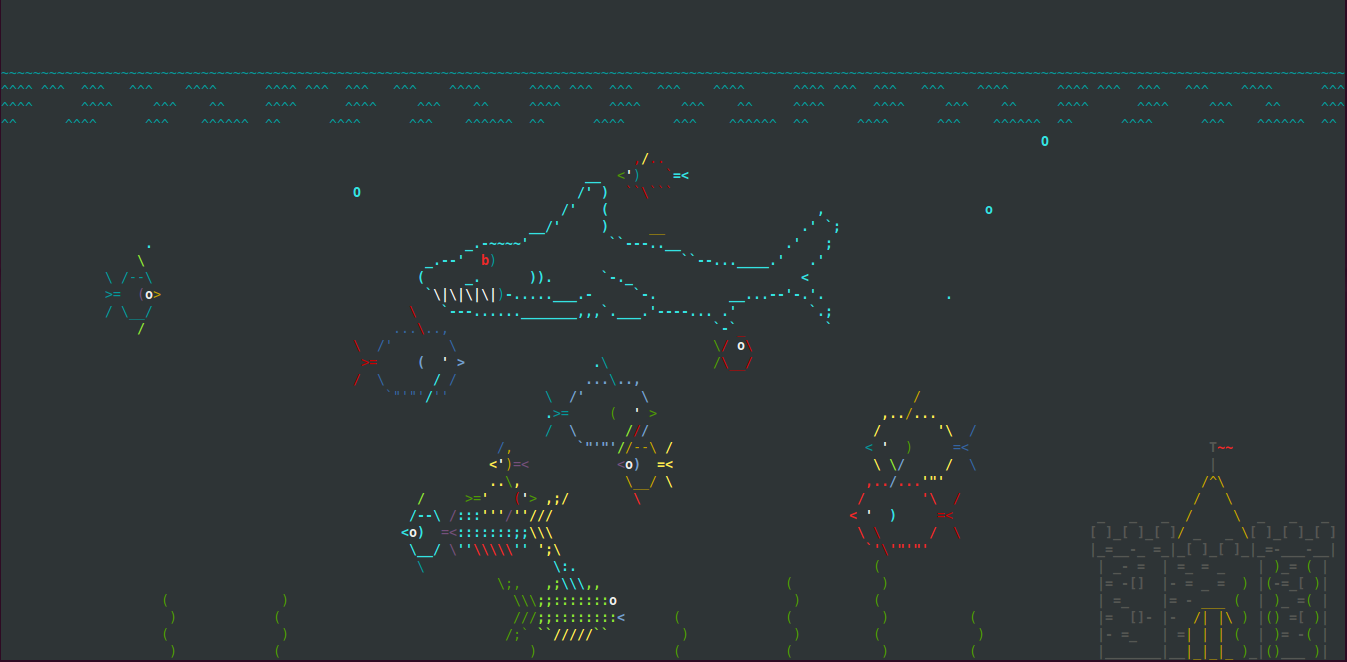
\includegraphics[width=\textwidth]{c2_perl_example_01.png}
  \end{figure}
\end{frame}

\begin{frame}
  \frametitle{Perl | 应用 | Frozen Bubble}
  \begin{figure}
    \centering
    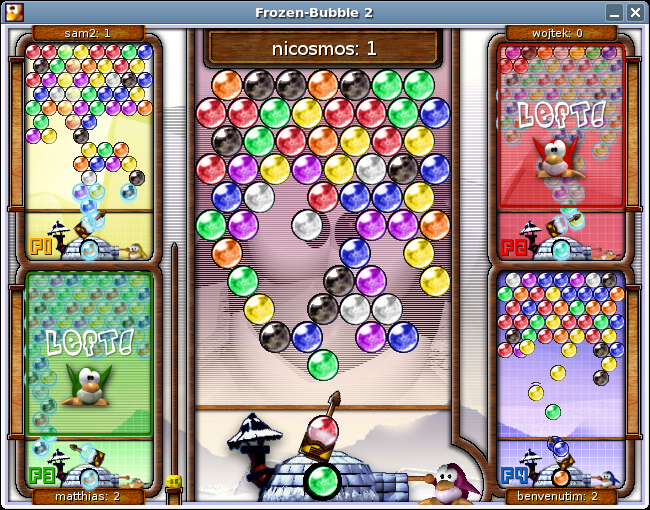
\includegraphics[width=0.8\textwidth]{c2_perl_example_12.png}
  \end{figure}
\end{frame}

\begin{frame}
  \frametitle{Perl | 应用 | ack}
  \begin{figure}
    \centering
    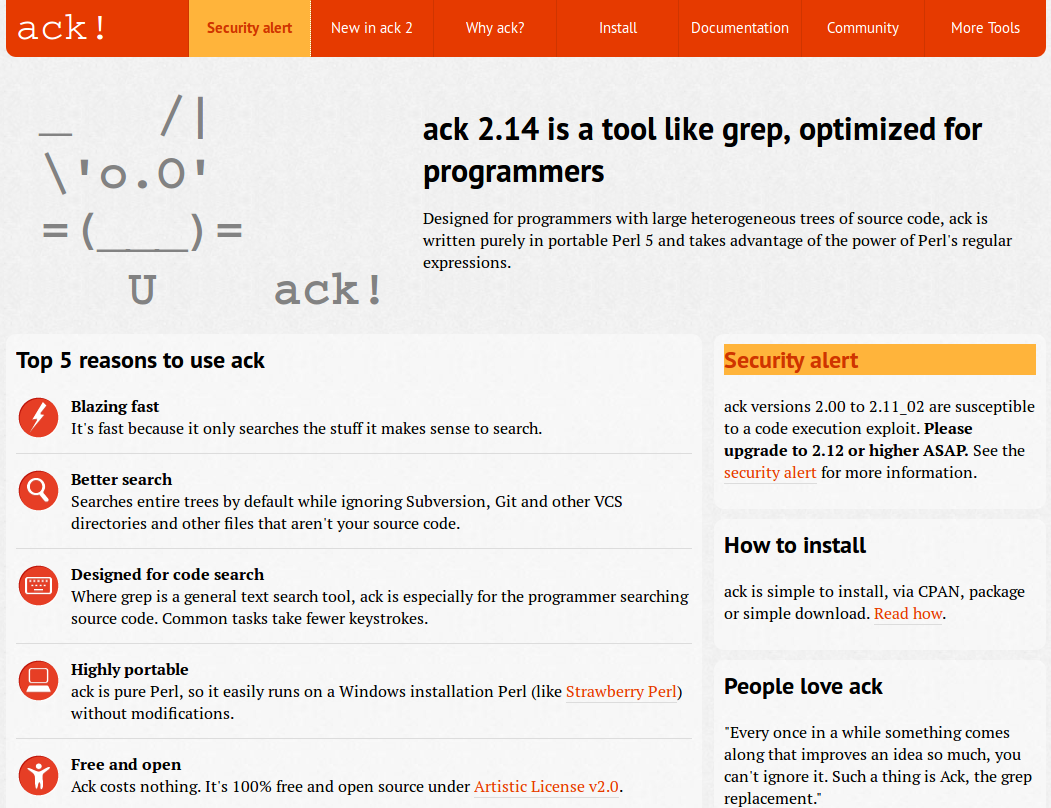
\includegraphics[width=0.85\textwidth]{c2_perl_example_11.png}
  \end{figure}
\end{frame}

\begin{frame}
  \frametitle{Perl | 应用 | Bugzilla}
  \begin{figure}
    \centering
    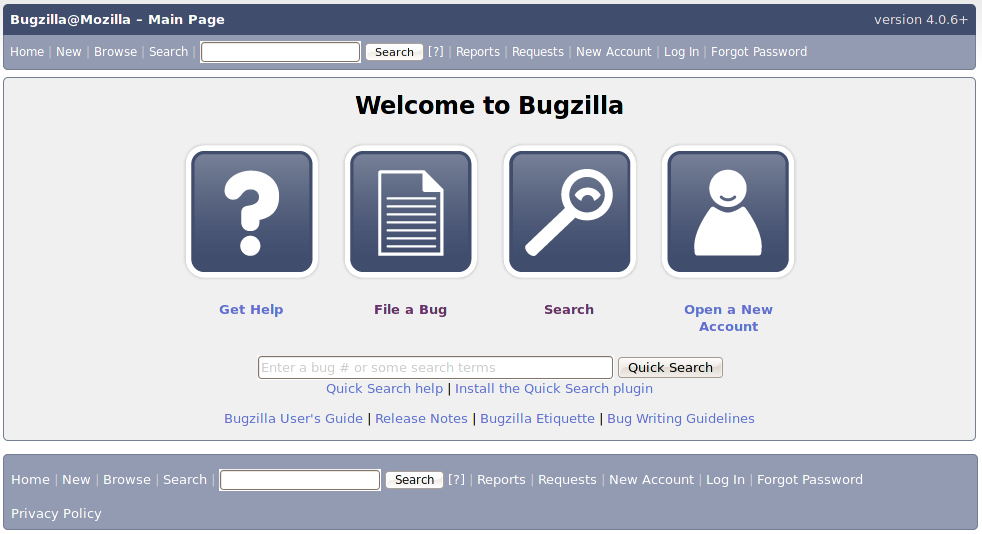
\includegraphics[width=\textwidth]{c2_perl_example_03.png}
  \end{figure}
\end{frame}

\begin{frame}
  \frametitle{Perl | 应用 | Webmin}
  \begin{figure}
    \centering
    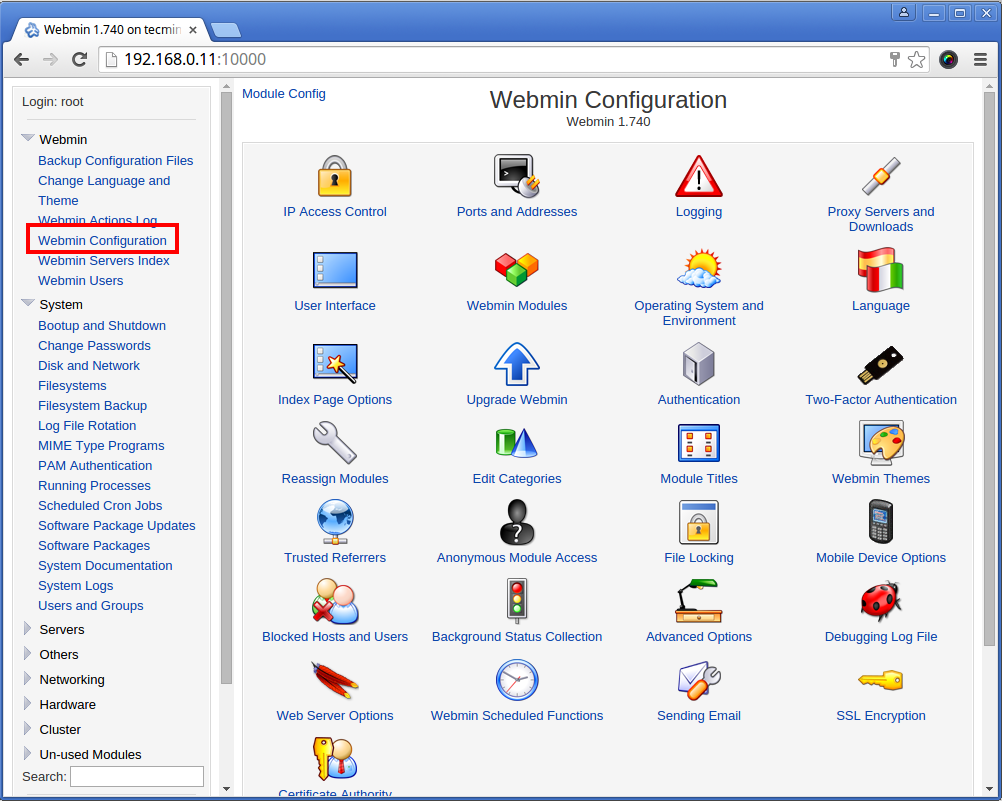
\includegraphics[width=0.8\textwidth]{c2_perl_example_04.png}
  \end{figure}
\end{frame}

\begin{frame}
  \frametitle{Perl | 应用 | Circos}
  \begin{figure}
    \centering
    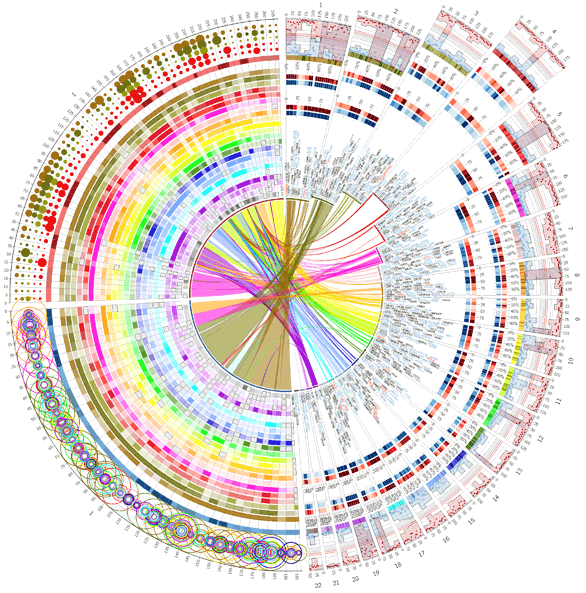
\includegraphics[width=0.65\textwidth]{c2_perl_example_07.png}
  \end{figure}
\end{frame}

\begin{frame}
  \frametitle{Perl | 标志}
  \begin{figure}
    \centering
    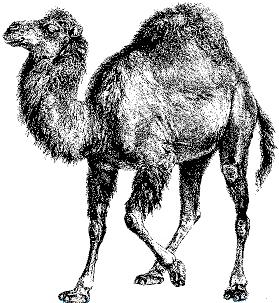
\includegraphics[width=3.3cm]{c2_perl_logo_01.jpg}
    \hspace{0.1cm}
    
\includegraphics[width=3.5cm]{c2_perl_logo_02.png}
    \hspace{0.1cm}
    
\includegraphics[width=4.5cm]{c2_perl_perl6.png}
  \end{figure}
  \begin{figure}
    \centering
    
\includegraphics[width=8cm]{c2_perl_logo_03.jpg}
  \end{figure}
\end{frame}

\begin{frame}
  \frametitle{Perl | 中心思想}
  \begin{itemize}
    \item \alert{TMTOWTDI}:There's More Than One Way To Do It. 不只一种方法来做一件事。发音为“Tim Toady”。
    \item TIMTOWTDIBSCINABTE:There's more than one way to do it, but sometimes consistency is not a bad thing either.  不只一种方法来做一件事,但有时保持一致也不错。发音为“Tim Toady Bicarbonate”。
    \item Easy things should be easy, and hard things should be possible. 简单的事情应该是简单的,复杂的事情应该变得可能。
  \end{itemize}
\end{frame}

\begin{frame}
  \frametitle{Perl | 优缺点}
  \begin{block}{优点}
    \begin{itemize}
      \item 很容易:容易使用,但学习Perl并不简单(入门容易精通难)
      \item 几乎不受限制:几乎没有什么事是Perl办不到的
      \item 速度通常很快
    \end{itemize}
  \end{block}
  \pause
  \begin{block}{缺点}
    \begin{itemize}
      \item 灵活、随意和“过度”的冗余语法
      \item write-only:代码有点难看,令人难以阅读
      \item 解释器耗费资源
    \end{itemize}
  \end{block}
\end{frame}

\begin{frame}[fragile]
  \frametitle{Perl | 优缺点 | JAPH}
  \vspace{-1.5em}
\begin{lstlisting}[basicstyle=\small\tt]
#JAPH(Just another Perl hacker) program without obfuscation:
print "Just another Perl hacker,";

#Embedding JAPH in opaque code:
$_='987;s/^(\d+)/$1-1/e;$1?eval:print"Just another Perl hacker,"';eval;

#Decoding JAPH from a transposed string literal:
$_="krJhruaesrltre c a cnP,ohet";$_.=$1,print$2while s/(..)(.)//;

#Appearing as if it does something completely unrelated to printing JAPH:
$_ = "wftedskaebjgdpjgidbsmnjgc";
tr/a-z/oh, turtleneck Phrase Jar!/; print;
\end{lstlisting}
\end{frame}

\begin{frame}
  \frametitle{Perl | 优缺点 | JAPH}
  \begin{figure}
    \centering
    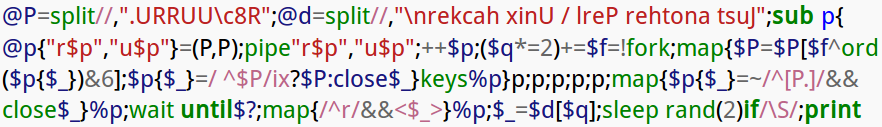
\includegraphics[width=0.9\textwidth]{c2_perl_japh_01.png}\\
    \vspace{1em}
    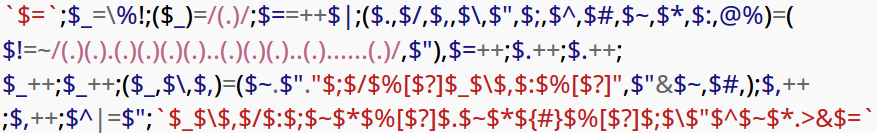
\includegraphics[width=0.9\textwidth]{c2_perl_japh_02.png}\\
    \vspace{1em}
    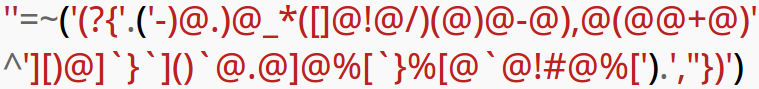
\includegraphics[width=0.9\textwidth]{c2_perl_japh_03.png}
  \end{figure}
\end{frame}

\begin{frame}
  \frametitle{Perl | 优缺点 | JAPH}
  \begin{figure}
    \centering
    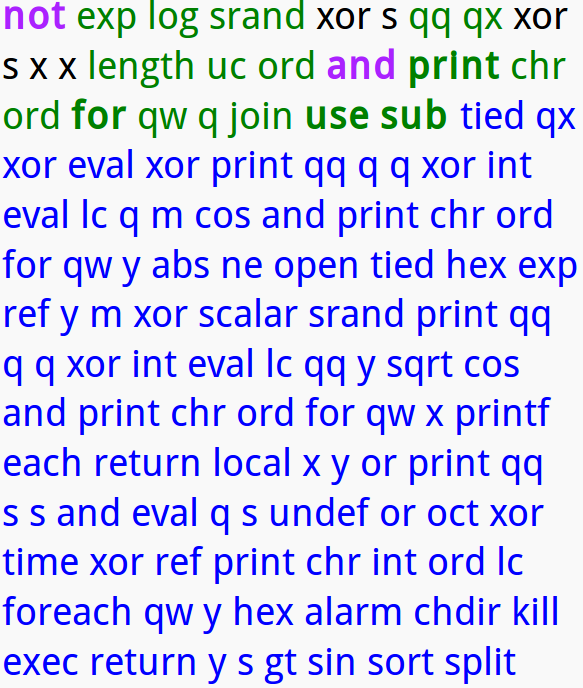
\includegraphics[width=0.51\textwidth]{c2_perl_japh_04.png}
    \quad
    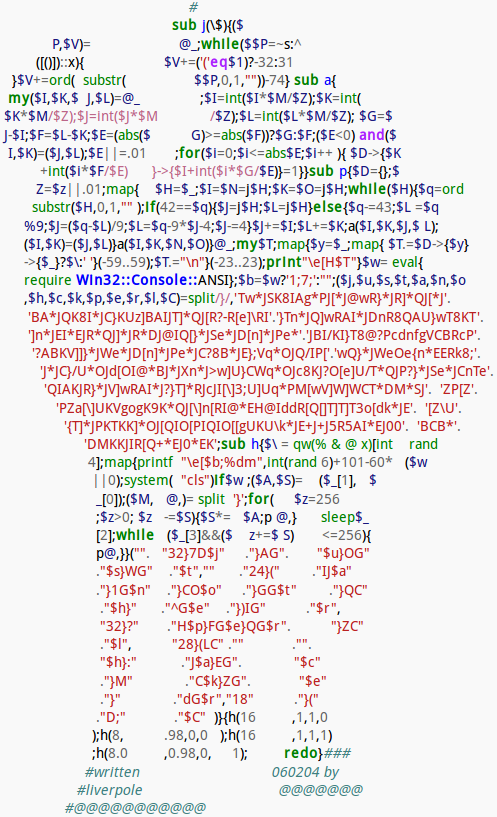
\includegraphics[width=0.365\textwidth]{c2_perl_japh_05.png}
  \end{figure}
\end{frame}

\begin{frame}[fragile]
  \frametitle{Perl | 优缺点 | JAPH}
  \vspace{-1em}
\begin{lstlisting}[language=Perl,basicstyle=\scriptsize\tt]
                        #!/usr/bin/perl
                          use strict;

                     my$f=           $[;my
                   $ch=0;sub       l{length}
                 sub r{join"",   reverse split
                ("",$_[$[])}sub ss{substr($_[0]
                ,$_[1],$_[2])}sub be{$_=$_[0];p
                 (ss($_,$f,1));$f+=l()/2;$f%=l 
                  ();$f++if$ch%2;$ch++}my$q=r
                   ("\ntfgpfdfal,ce?bngbjn".    
                    "axfvxf"); $_=$q; $q=~
                      tr/f[a-z]/ [l-za-k]
                        /;my@ever=1..&l
                          ;my$mine=$q
                            ;sub p{
                             print
                              @_;
                               }

                       be $mine for @ever
\end{lstlisting} 
\end{frame}

\begin{frame}
  \frametitle{Perl | 优势}
  \begin{block}{易于编程}
    Perl的一些特性,使得解决常见的生物信息学问题非常容易。
  \end{block}
  \pause
  \begin{block}{快速成型}
    程序员可以快速写出实用的Perl程序(尤其是频率低或需频繁修改)。
  \end{block}
  \pause
  \begin{block}{可移植性好}
    可以在不同的计算机、操作系统上运行Perl程序。
  \end{block}
  \pause
  \begin{block}{速度还可以}
    先用Perl编写程序,再用C重写需要提速的部分。(\alert{开发时间远比运行时间宝贵!})
  \end{block}
  \pause
  \begin{block}{程序容易维护}
    程序是死的,人是活的。(\alert{维护程序不比编写程序容易。})
  \end{block}
\end{frame}

\begin{frame}
  \frametitle{Perl | 版本}
  \begin{block}{Perl5}
    \begin{itemize}
      \item 1994年——至今
      \item 最新版:v5.30.0(2019-05-22)
    \end{itemize}
  \end{block}
  \pause
  \begin{block}{Perl6\textcolor{gray}{(一种全新的编程语言)}}
    \begin{itemize}
      \item 2000年——至今(2015-12-25发布v1.0)
      \item 最新版:Rakudo Star 2019.03(2019-03-30)
    \end{itemize}
  \end{block}
  \pause
  \begin{block}{版本选择}
    \begin{itemize}
      \item 推荐Perl5(关注Perl6):兼容性好,稳定,模块丰富,资源丰富,……
      \item (Perl5 vs. Perl6) vs. (Python2 vs. Python3)
    \end{itemize}
  \end{block}
\end{frame}

\begin{frame}[fragile]
  \frametitle{Perl | 版本 | Perl5 vs. Perl6}
  \begin{block}{Inline::Perl5}
    Use Perl 5 code in a Perl 6 program.\\
    Let you run all 170,000+ Perl 5 modules while letting you get on with new Perl 6 development.
  \end{block}
  \pause
  \begin{block}{Inline::Perl6}
    Use Perl 6 in Perl 5 code.
  \end{block}
  \pause
  \begin{block}{Blue Tiger}
    Perl 5 to Perl 6 Translator.
  \end{block}
  \pause
  \begin{block}{Perl::ToPerl6}
    Transmogrify Perl5 code into Perl6.\\
    An extensible framework for creating and applying coding standards to Perl source code.
  \end{block}
\end{frame}

\begin{frame}[fragile]
  \frametitle{Perl | 安装}
  \begin{block}{\alert{查看版本}确认是否已安装}
\begin{lstlisting}[language=bash]
perl -v
\end{lstlisting}
  \end{block}
  \pause
  \begin{block}{官网}
    \href{https://www.perl.org/}{https://www.perl.org/}
  \end{block}
  \pause
  \begin{block}{Unix/Linux/Mac OS X}
    已经预装!
  \end{block}
  \pause
  \begin{block}{Windows}
    \begin{itemize}
      \item \href{http://strawberryperl.com/}{Strawberry Perl}【推荐】
      \item \href{http://www.activestate.com/activeperl/downloads}{ActivePerl}
    \end{itemize}
  \end{block}
\end{frame}

\begin{frame}[fragile]
  \frametitle{Perl | 学习}
  \begin{block}{基本策略}
    基础毛坯,主题精装。(先学习基础知识,当需要时再学习相关主题。)\\
80/20定律:Perl里面80\%的功能可以用文档中20\%的部分加以描述,而另外20\%的功能却需要占据其他80\%的篇幅。(扩展:80\%的任务可以用20\%的知识解决,20\%的任务则需要剩余80\%的知识。)
  \end{block}
  \pause
  \begin{block}{各种资源}
    \begin{itemize}
      \item 自带文档(\verb|man perl|)
      \item 在线文档
      \item 新闻组
      \item FAQs
      \item 邮件列表
      \item 书籍
      \item ……
    \end{itemize}
  \end{block}
\end{frame}

\begin{frame}
  \frametitle{Perl | 学习 | 书籍}
  \begin{block}{生物信息学角度}
    \textit{\alert{Beginning}} $\Longrightarrow$ \textit{Mastering Perl for Bioinformatics}
  \end{block}
  \begin{figure}
    \centering
    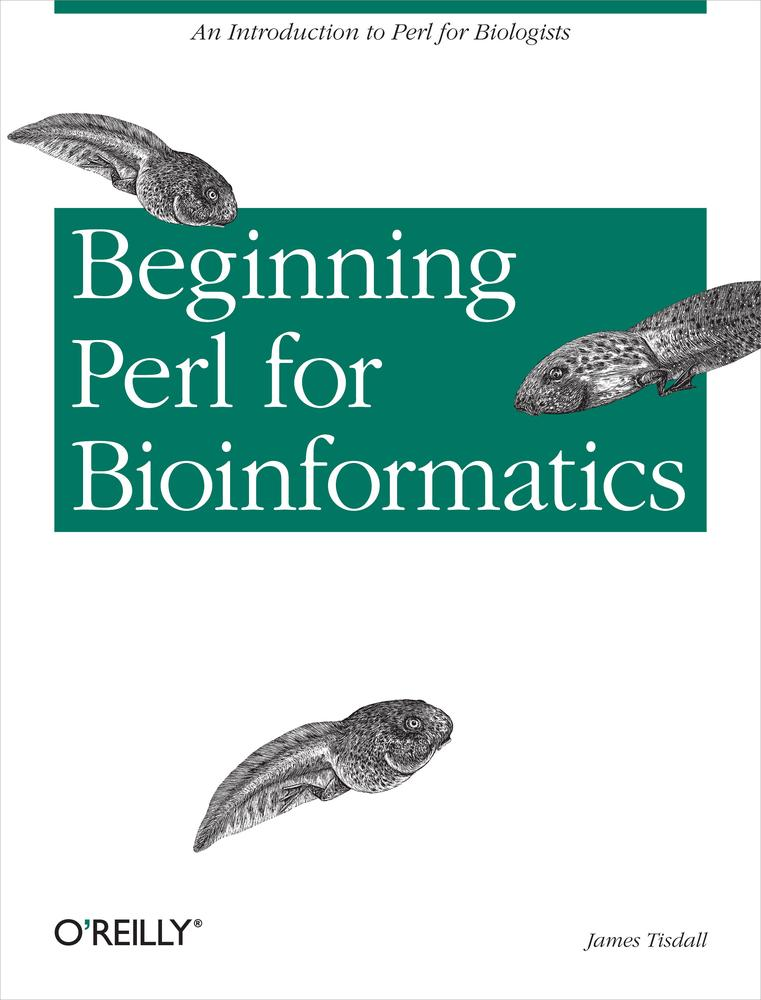
\includegraphics[width=4.5cm]{c2_perl_bpfb.jpg}
    \hspace{1em}
    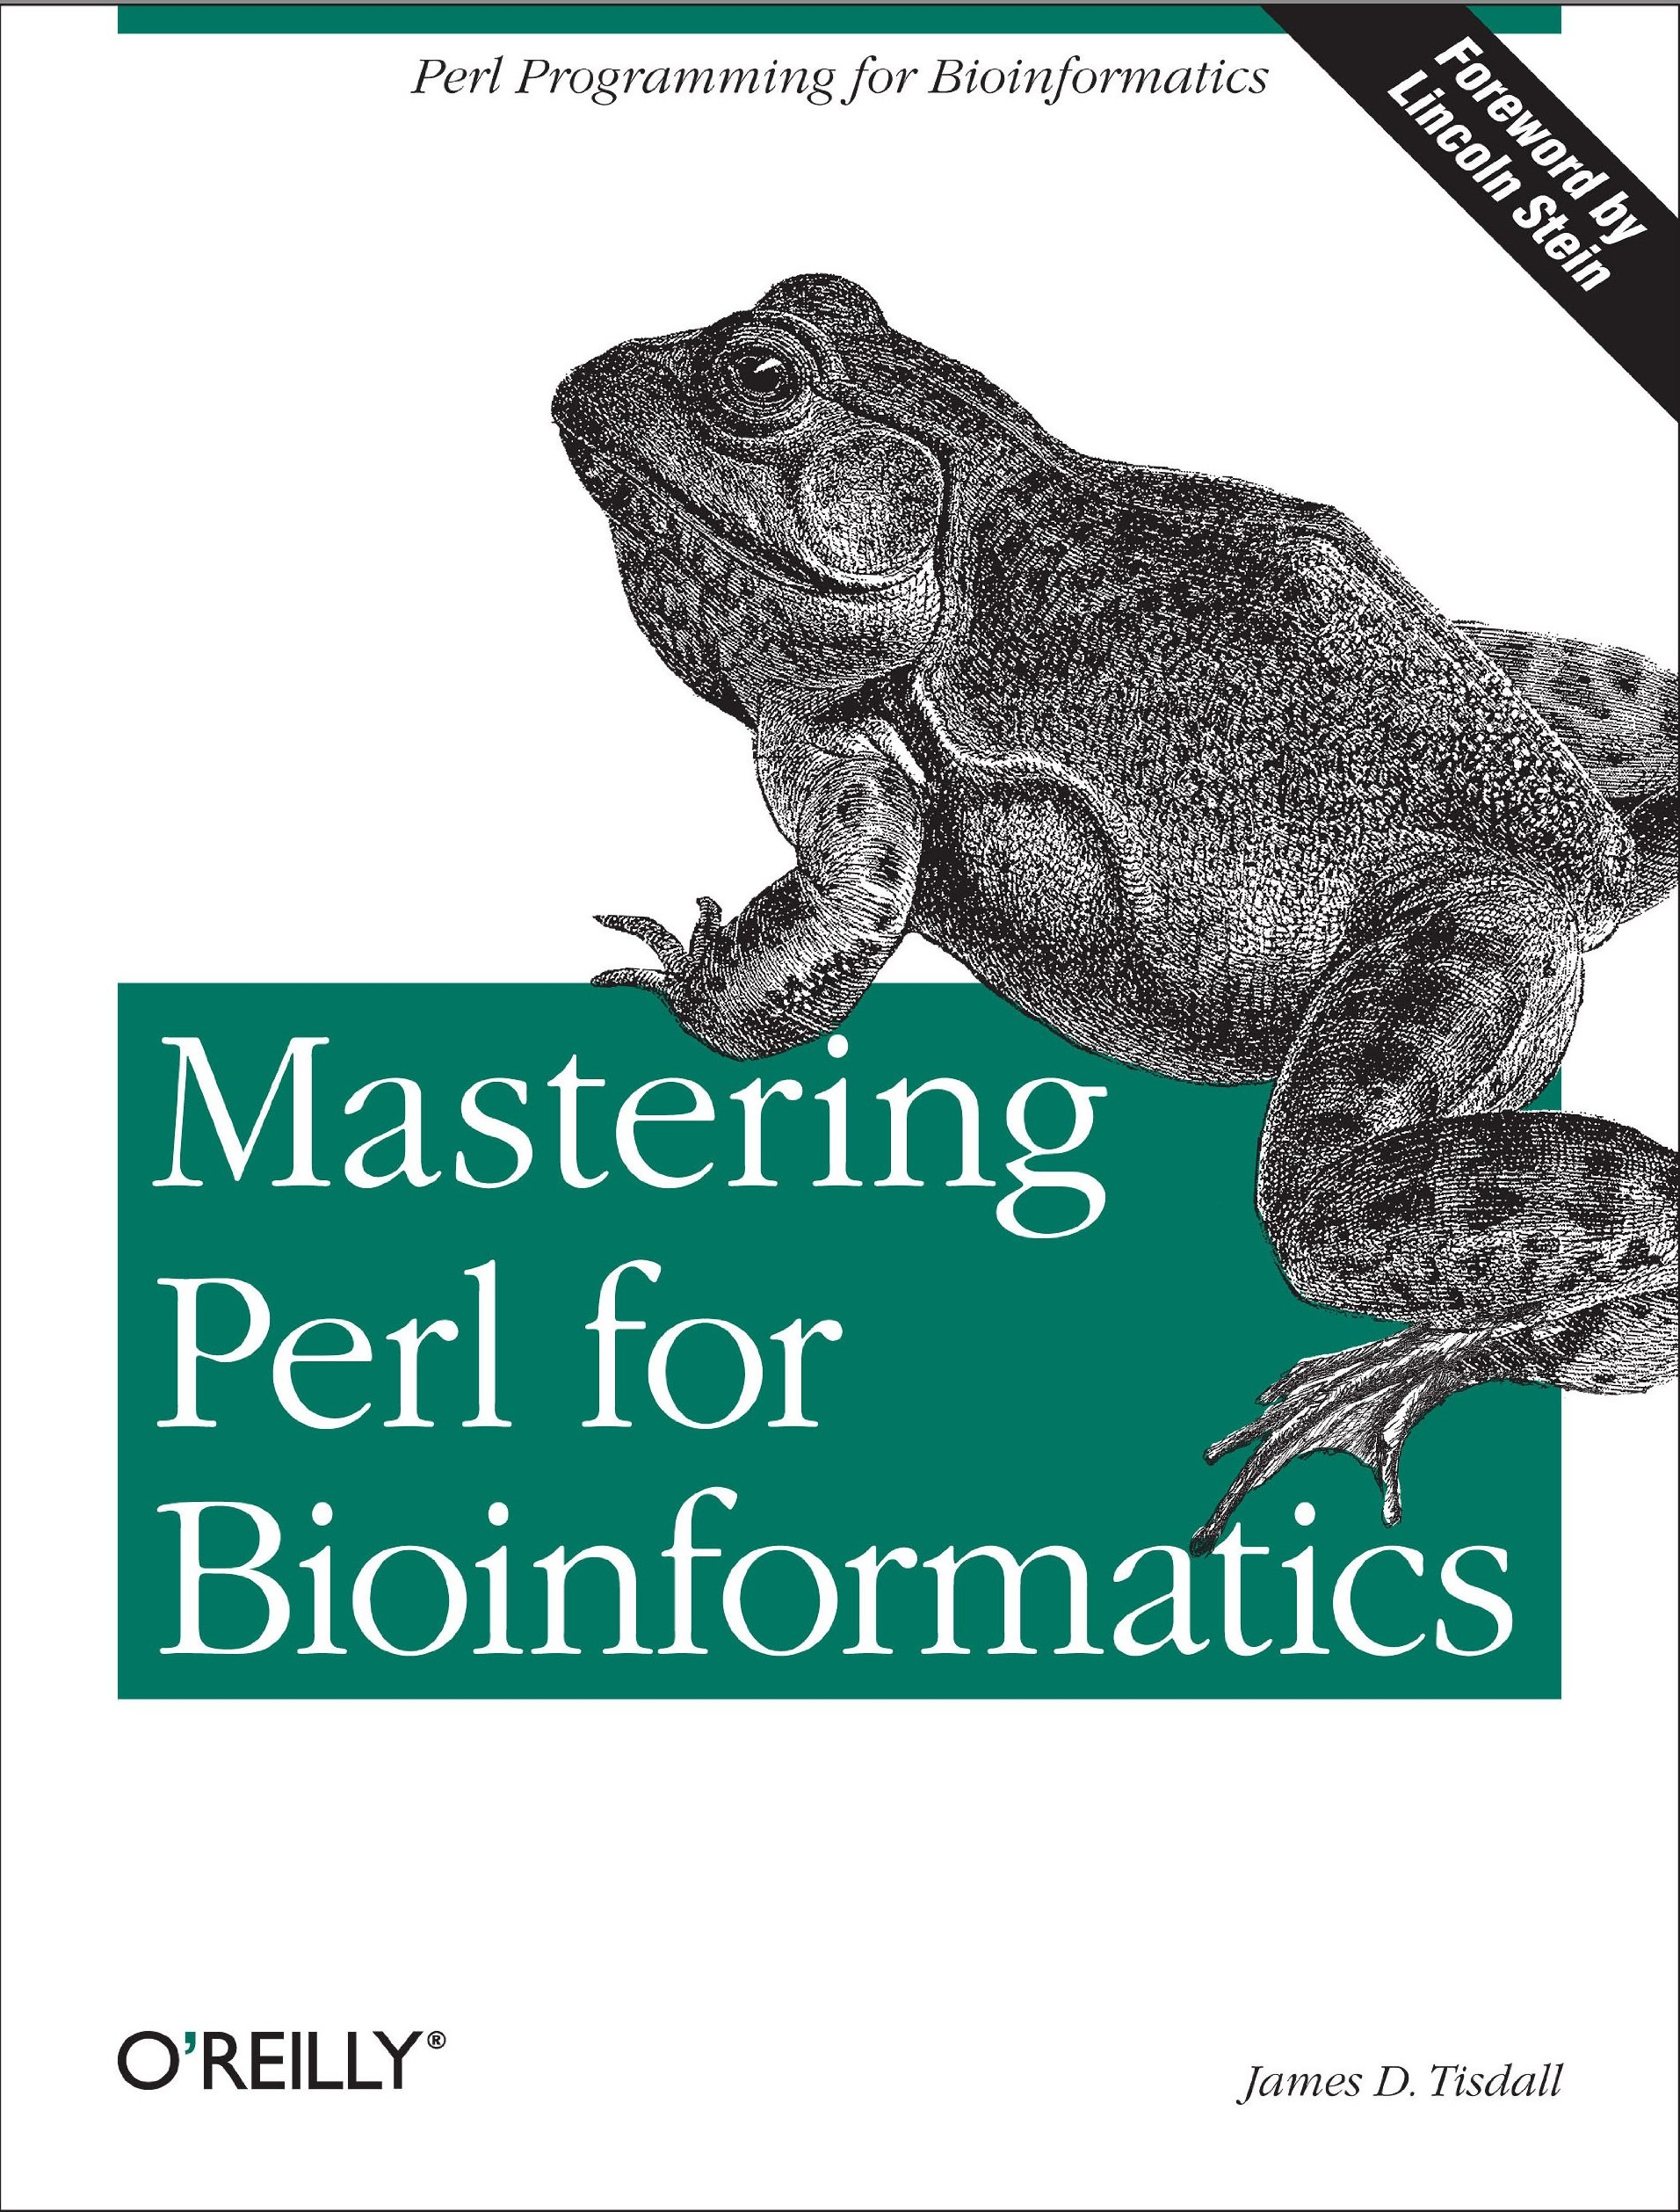
\includegraphics[width=4.5cm]{c2_perl_mpfb.jpg}
  \end{figure}
\end{frame}

\begin{frame}
  \frametitle{Perl | 学习 | 书籍}
  \begin{block}{编程语言角度:代号}
小骆驼 $\Rightarrow$ 羊驼书 $\Rightarrow$ 小羊驼母亲和她的孩子 $\Rightarrow$ 大骆驼 $\Rightarrow$ 黑豹书
  \end{block}
  \pause
  \begin{block}{英文名}
    \textit{Learning Perl} $\Rightarrow$ \textit{Intermediate Perl} $\Rightarrow$ \textit{Mastering Perl} $\Rightarrow$ \textit{Programming Perl} $\Rightarrow$ \textit{Advanced Perl Programming}
  \end{block}
  \pause
  \begin{block}{中文名}
    \alert{《Perl语言入门》} $\Rightarrow$ 《Perl进阶》 $\Rightarrow$ 《精通Perl》 $\Rightarrow$ 《Perl语言编程》 $\Rightarrow$ 《高级Perl编程》
  \end{block}
  \pause
\end{frame}

\begin{frame}
  \frametitle{Perl | 学习 | 书籍}
  \begin{figure}
    \centering
    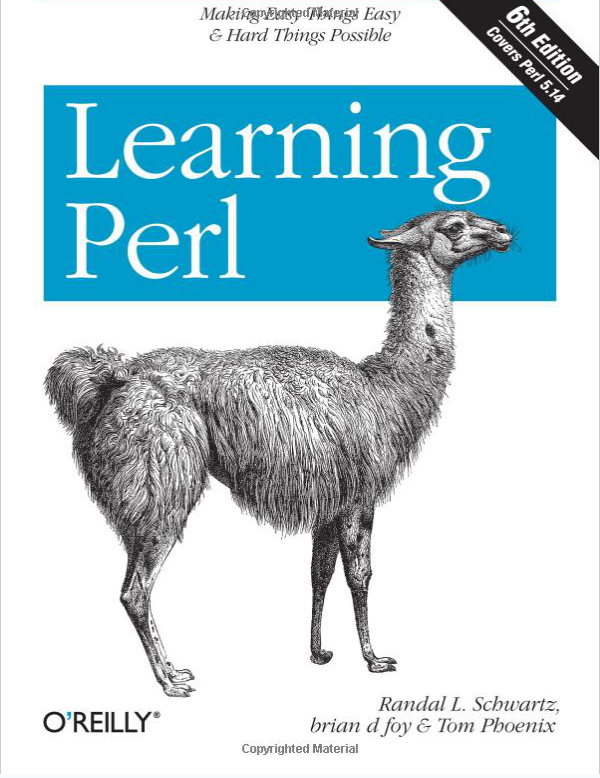
\includegraphics[width=3cm]{c2_perl_lp.png}
    \qquad
    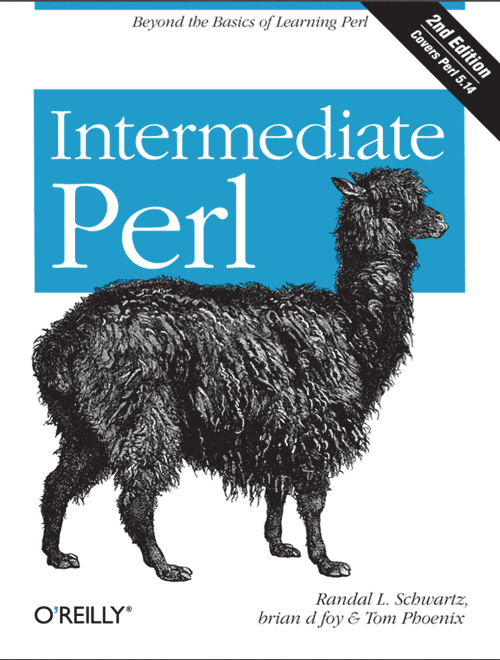
\includegraphics[width=3cm]{c2_perl_ip.png}
    \qquad
    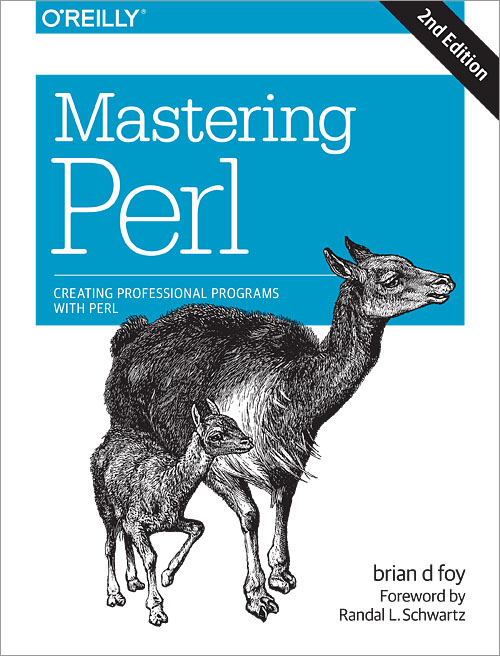
\includegraphics[width=3cm]{c2_perl_mp.jpg}\\
    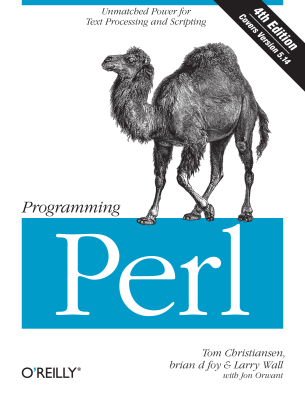
\includegraphics[width=3cm]{c2_perl_pp.png}
    \hspace{2cm}
    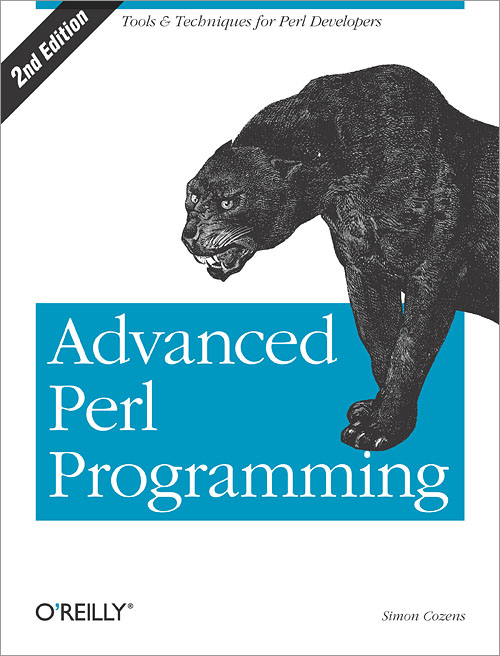
\includegraphics[width=3cm]{c2_perl_app.jpg}
  \end{figure}
\end{frame}

\begin{frame}
  \frametitle{书籍 | Perl}
  \begin{columns}
    \column{0.4\textwidth}
  \begin{block}{中文名}
    \begin{itemize}
      \item \alert{《Perl入门经典》}
      \item 《高阶Perl》
      \item 《Perl高效编程》
      \item 《Perl最佳实践》
      \item \textit{Perl Cookbook}
    \end{itemize}
  \end{block}
    \column{0.5\textwidth}
  \begin{block}{英文名}
    \begin{itemize}
      \item \textit{Beginning Perl}
      \item \textit{Higher-Order Perl}
      \item \textit{Effective Perl Programming}
      \item \textit{Perl Best Practices}
      \item \textit{Perl Cookbook}
    \end{itemize}
  \end{block}
\end{columns}
\end{frame}

\begin{frame}
  \frametitle{书籍 | Perl}
  \begin{figure}
    \centering
    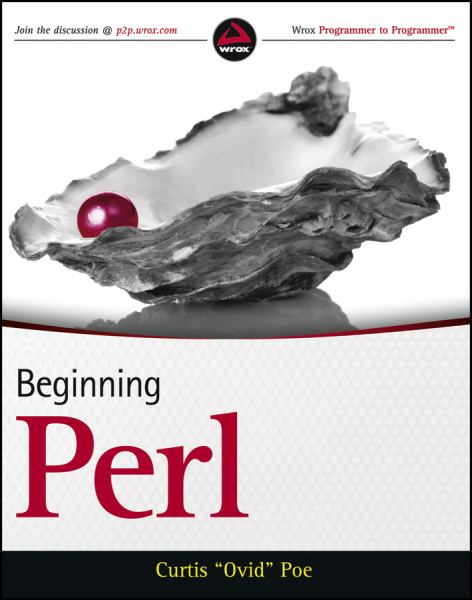
\includegraphics[height=3.8cm]{c1_book_perl_bp.jpg}\qquad
    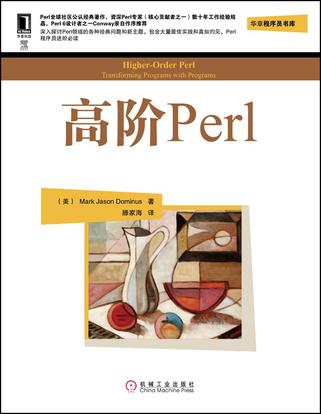
\includegraphics[height=3.8cm]{c1_book_perl_hop.jpg}\\
    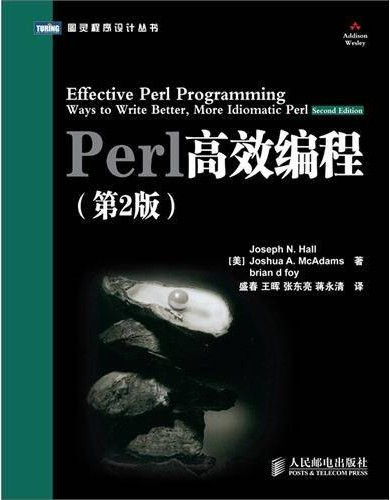
\includegraphics[height=3.85cm]{c1_book_perl_epp.jpg}\quad
    
\includegraphics[height=3.85cm]{c1_book_perl_pbp.jpg}\quad
    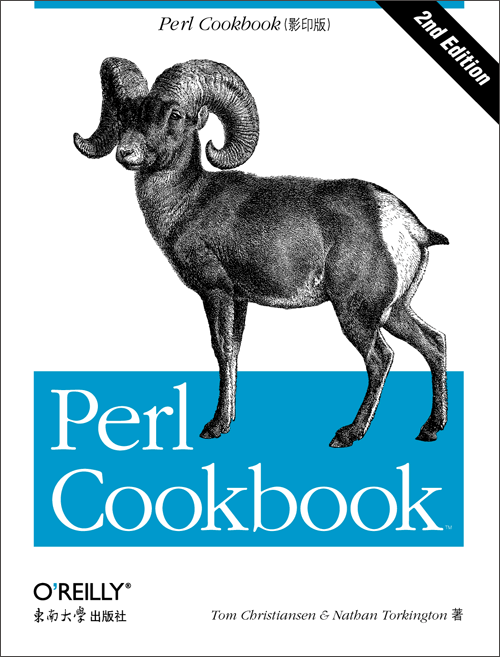
\includegraphics[height=3.85cm]{c1_book_perl_pc.png}
  \end{figure}
\end{frame}

\begin{frame}[fragile]
  \frametitle{Perl | \alert{语法}}
  \vspace{-1em}
\begin{lstlisting}[language=Perl]
#!/usr/bin/perl
# Classic "Hello World" as done with Perl

use strict;
use warnings;

print "Hello World!\n";
\end{lstlisting}
\pause
\begin{lstlisting}
# Step 1:编写脚本
vim hello.pl
# Step 2:修改权限
chmod 755 hello.pl
# Step 3:运行脚本
perl hello.pl
./hello.pl
\end{lstlisting}
\end{frame}

\begin{frame}[fragile]
  \frametitle{Perl | 文本编辑器}
  \begin{block}{Vim插件}
    \href{https://github.com/vim-scripts/perl-support.vim}{perl-support.vim}: Perl IDE -- Write and run Perl-scripts using menus and hotkeys.
  \end{block}
  {\footnotesize
  \begin{itemize}
    \item insert various types of comments
    \item insert complete but empty statements (e.g. `if \verb|{}| else \verb|{}|' )
    \item insert often used code snippets (e.g. declarations, the opening of files, .. )
    \item insert the names of file tests, character classes, special Perl-variables and POSIX-signals
    \item read, write, maintain your own code snippets in a separate directory
    \item run scripts or run syntax check from within the editor
    \item show compilation erros in a quickfix window; navigate with hotkeys 
    \item read perldoc for functions and modules 
    \item run perltidy / run the profiler SmallProf
    \item test / explain regular expressions (needs Vim with Perl interface)
  \end{itemize}
}
\end{frame}

\begin{frame}[fragile]
  \frametitle{Perl | 语法检查}
  \begin{block}{\alert{检查语法}}
\begin{lstlisting}[language=bash]
perl -c script.pl
\end{lstlisting}
  \end{block}
  \pause
  \begin{block}{常见错误}
    \begin{itemize}
      \item Missing right curly or square bracket: 括号不匹配
      \item 语句末尾少了分号
      \item 关键字(内置函数)拼写错误
      \item 变量类型符号(\verb|$@%|)错误/变量名拼写错误
      \item ……
    \end{itemize}
  \end{block}
\end{frame}

\begin{frame}[fragile]
  \frametitle{Perl | 格式化 | \alert{perltidy}}
  \vspace{-1em}
\begin{lstlisting}[language=bash]
# 安装perltidy
sudo apt install perltidy
#sudo apt-get install perltidy

# 保留原始文件,格式化后的文件为*.tdy
perltidy script.pl

# 备份原始文件为*.bak,格式化后的文件使用原文件名
perltidy -b script.pl

# perltidy使用帮助
man perltidy
perltidy -h
\end{lstlisting} 
\end{frame}

\begin{frame}[fragile]
  \frametitle{Perl | 格式化 | 前}
  \vspace{-1em}
\begin{lstlisting}[language=Perl]
#!/usr/bin/perl 

use strict;use warnings;use utf8;

for(my$i=1;$i<=9;$i++){for(my$j=1;$j<=$i;$j++){print"$j"."x"."$i"."=".$i*$j;
if($j==$i){print"\n";}else{print"\t";}}}
\end{lstlisting} 
\end{frame}

\begin{frame}[fragile]
  \frametitle{Perl | 格式化 | \alert{后}}
  \vspace{-1em}
\begin{lstlisting}[language=Perl,basicstyle=\small\tt]
#!/usr/bin/perl 

use strict;
use warnings;
use utf8;

for ( my $i = 1 ; $i <= 9 ; $i++ ) {
    for ( my $j = 1 ; $j <= $i ; $j++ ) {
        print "$j" . "x" . "$i" . "=" . $i * $j;
        if   ( $j == $i ) { print "\n"; }
        else              { print "\t"; }
    }
}
\end{lstlisting} 
\end{frame}

\section{变量}
\begin{frame}[fragile]
  \frametitle{变量}
  \begin{block}{变量}
    Perl是一种无类型语言(untyped),换句话说,在语言层面上,Perl和大多数编程语言不同,不把变量分成整数、字符、浮点数等等,而只有一种能接受各种类型数据的“无类型”变量。\\
    Perl中各种变量的运算也很自由,数和含有数的字符串是等效的,可以把数字字符串参与数学计算,也可以反之,让数字参与字符串的构成和操作。
  \end{block}
  \pause
  \begin{block}{\alert{类型}}
    \begin{itemize}
      \item 标量:scalar;只包含一个元素的变量;以 \verb|$| 开头;类比“个体”
      \item 数组:array;含有任意数量元素的变量,以其存储顺序作为索引;以 \verb|@| 开头;类比“队列”
      \item 散列:hash,associative array(关联数组);像字典一样,把不同的变量按照它们的逻辑关系组织起来,并以作为“键”的变量进行索引;以 \verb|%| 开头;类比“字典”
    \end{itemize}
  \end{block}
\end{frame}

\subsection{标量}
\begin{frame}[fragile]
  \frametitle{变量 | 标量 | \alert{语法}}
  \vspace{-1em}
\begin{lstlisting}[language=Perl]
# 标量:$scalar

# 字符串,双引号
$name = "Paul";

# 字符串,单引号
$where_to_find_him = 'http://www.weinstein.org';

# 数字,无引号
$age = 29;
\end{lstlisting}
\end{frame}

\subsection{数组}
\begin{frame}
  \frametitle{变量 | 数组 | 简介}
  \begin{figure}
    \centering
    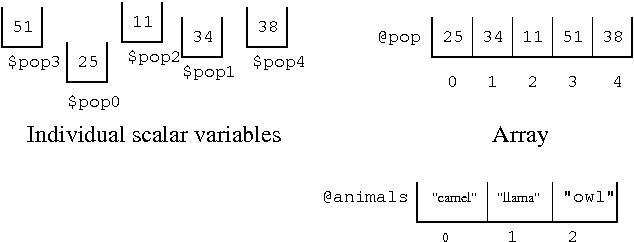
\includegraphics[width=10cm]{c2_perl_array_01.jpg}
  \end{figure}
\end{frame}

\begin{frame}[fragile]
  \frametitle{变量 | 数组 | \alert{语法}}
  \vspace{-1em}
\begin{lstlisting}[language=Perl]
# 数组:@array
# 索引值从0开始

# 字符串
@authors = ("Paul", "Joe", "Jeremy", "Harley");
$authors[4] = "Tom";

# 数字
@list = (1, 2, 3, 4);

# 解引用:$array[index]
$authors[4] # Tom
$list[0] # 1
\end{lstlisting}
\end{frame}

\begin{frame}
  \frametitle{变量 | 数组 | \alert{操作}}
  \begin{figure}
    \centering
    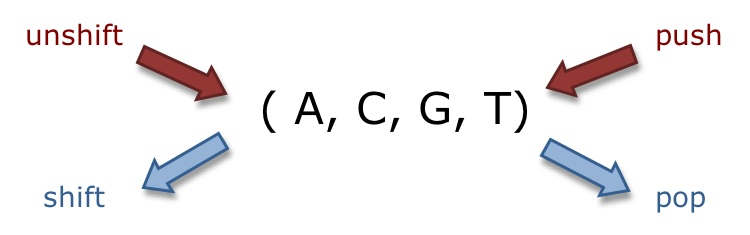
\includegraphics[width=10cm]{c2_perl_array_02.jpg}
    \vspace{0.5cm}
    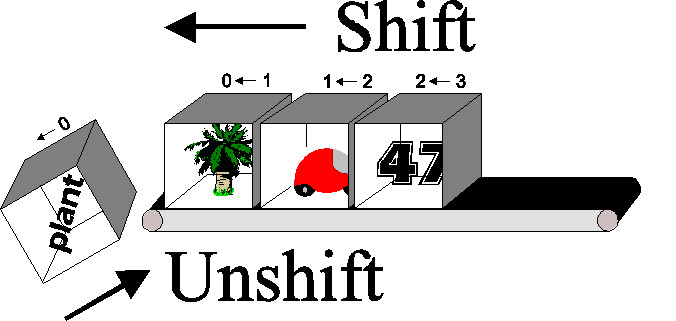
\includegraphics[width=5.5cm]{c2_perl_array_03.png}
    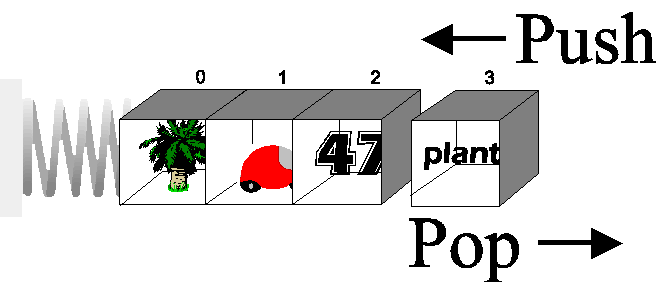
\includegraphics[width=5.5cm]{c2_perl_array_04.png}
  \end{figure}
\end{frame}

\subsection{散列}
\begin{frame}
  \frametitle{变量 | 散列 | 简介}
  \begin{figure}
    \centering
    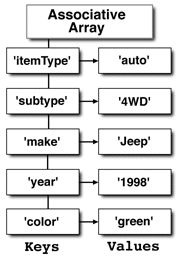
\includegraphics[width=2.8cm]{c2_perl_hash_01.png}\qquad
    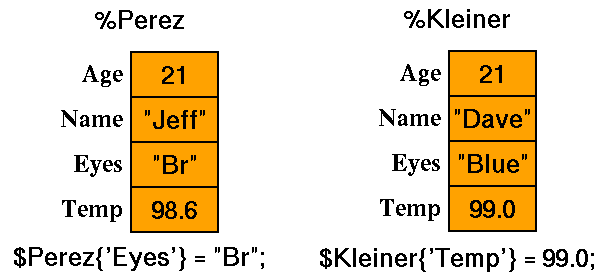
\includegraphics[width=8.2cm]{c2_perl_hash_02.png}
  \end{figure}
\end{frame}

\begin{frame}[fragile]
  \frametitle{变量 | 散列 | \alert{语法}}
  \vspace{-1em}
\begin{lstlisting}[language=Perl]
# 散列:%hash

# 创建散列
%person = (
name => 'Paul',
age => '29',
url => 'http://www.weinstein.org',
)
# 友情提示:注意最后一个元素(括号前的最后一行)的末尾

# 提取键值:$hash{key}
$person{"age"} # 29
\end{lstlisting}
\end{frame}

\subsection{内置变量}
\begin{frame}[fragile]
  \frametitle{变量 | 内置变量}
  \begin{figure}
    \centering
    
\includegraphics[width=11cm]{c2_perl_buildin_01.jpg}
  \end{figure}
  \begin{center}
其中重要/常用的几个\alert{内置变量}:\verb|$_|,\verb|$!|,\verb|$0|,\verb|@ARGV|,\verb|@_|
  \end{center}
\end{frame}

\section{操作符}
\begin{frame}[fragile]
  \frametitle{操作符 | \alert{数字操作符}}
  \begin{table}
    \centering
    \rowcolors[]{1}{blue!20}{blue!10}
    \begin{tabularx}{0.7\textwidth}{cX}
      \hline
      \rowcolor{blue!50}操作符 & 含义\\
      \hline
      \verb|+| & 加法\\
      \verb|-| & 减法\\
      \verb|*| & 乘法\\
      \verb|/| & 除法\\
      \verb|**| & 乘幂,乘方\\
      \% & 取模,取余\\
      \hline
      \verb|<|  & 小于\\
      \verb|>|  & 大于\\
      \verb|==|  & 等于\\
      \verb|<=|  & 小于等于\\
      \verb|>= |  & 大于等于\\
      \verb|!=|  & 不等于\\
      \verb|<=>|  & 比较。\verb|a<=>b|:a等于b时返回0,a大于b时返回1,a小于b时返回-1\\
      \hline
    \end{tabularx}
  \end{table}
\end{frame}

\begin{frame}
  \frametitle{操作符 | \alert{字符串操作符}}
  \begin{table}
    \centering
    \rowcolors[]{1}{blue!20}{blue!10}
    \begin{tabularx}{0.7\textwidth}{cX}
      \hline
      \rowcolor{blue!50}操作符 & 含义\\
      \hline
      \verb|.| & 连接。\verb|"string1" . "string2"|\\
      \verb|x| & 重复。\verb|"string" x number|\\
      \verb|lt| & 小于\\
      \verb|gt| & 大于\\
      \verb|eq| & 等于\\
      \verb|le| & 小于等于\\
      \verb|ge| & 大于等于\\
      \verb|ne| & 不等于\\
      \verb|cmp| & 比较。类似于数字比较的 \verb|<=>|\\
      \hline
    \end{tabularx}
  \end{table}
\end{frame}

\begin{frame}
  \frametitle{操作符 | \alert{逻辑操作符}}
  \begin{table}
    \centering
    \rowcolors[]{1}{blue!20}{blue!10}
    \begin{tabularx}{0.5\textwidth}{cX}
      \hline
      \rowcolor{blue!50}操作符 & 含义\\
      \hline
      \verb|&&| & 逻辑AND,与\\
      \verb=||= & 逻辑OR,或\\
      \verb|!| & 逻辑NOT,非\\
      \verb|?=| & 条件操作符\\
      \hline
    \end{tabularx}
  \end{table}
\end{frame}

\begin{frame}
  \frametitle{操作符 | 文件测试操作符}
  \begin{table}
    \centering
    \rowcolors[]{1}{blue!20}{blue!10}
    \begin{tabularx}{0.7\textwidth}{cX}
      \hline
      \rowcolor{blue!50}操作符 & 含义\\
      \hline
      -r & 可读\\
      -w & 可写\\
      -x & 可执行\\
      -e & 存在\\
      -z & 存在但没有内容\\
      -s & 存在且有内容\\
      -f & 普通文件\\
      -d & 目录\\
      -l & 符号链接\\
      -T & 看起来像文本文件\\
      -B & 看起来像二进制文件\\
      -M & 最后被修改后至今的天数\\
      -A & 最后被访问后至今的天数\\
      -C & 最后inode变更后至今的天数\\
      \hline
    \end{tabularx}
  \end{table}
\end{frame}

\begin{frame}[fragile]
  \frametitle{操作符 | \alert{匹配操作符}}
  \begin{table}
    \centering
    \rowcolors[]{1}{blue!20}{blue!10}
    \begin{tabularx}{0.5\textwidth}{cX}
      \hline
      \rowcolor{blue!50}操作符 & 含义\\
      \hline
      \verb|=~| & 绑定操作符,匹配\\
      \verb|!~| & 绑定操作符,不匹配\\
      \verb|~~| & 智能匹配操作符\\
      \hline
    \end{tabularx}
  \end{table}
\end{frame}

\section{基本函数}
\begin{frame}[fragile]
  \frametitle{基本函数 | \alert{print, chomp}}
  \vspace{-1em}
\begin{lstlisting}[language=Perl]
# 向标准输出打印文本
print "Hello Again\n";

# 向一个具有文件句柄的文件打印文本
print FILE "Hello Again\n";
print $FILE "Hello Again\n";

# 打印变量的值
print "How are on this day, the " . $date . "?\n";
\end{lstlisting}
\pause
\begin{lstlisting}[language=Perl]
# 删除变量末尾的(多个)换行符,返回删除的换行符的个数
chomp $name;
chomp @authors;
\end{lstlisting}
\end{frame}

\begin{frame}[fragile]
  \frametitle{基本函数 | \alert{join, split}}
  \vspace{-1em}
\begin{lstlisting}[language=Perl]
# joining a number of strings togother with a colon delimiter
$fields = join ':', $data_field1, $data_field2, $data_field3;

# splitting a string into substrings
($field1, $field2) = split /:/, 'Hello:World', 2;

# splitting a scalar and creating an array
@fields = split /:/, $raw_data;
\end{lstlisting}
\end{frame}

\begin{frame}[fragile]
  \frametitle{基本函数 | \alert{open, close}}
  \vspace{-1em}
\begin{lstlisting}[language=Perl]
# open the file and slurp its contents into an array and then close the file
open(FILE, "/etc/passwd");
@filedata = <FILE>; #囫囵吞枣
close(FILE);

open my $IN, '<', $file_in or die "$0 : failed to open input file '$file_in' : $!\n";
while(<$IN>){ #细嚼慢咽
  chomp;
  #...actions...;
}
close $IN or warn "$0 : failed to close input file '$file_in' : $!\n";
\end{lstlisting}
\end{frame}

\begin{frame}[fragile]
  \frametitle{基本函数 | opendir, readdir, closedir}
  \vspace{-1em}
\begin{lstlisting}[language=Perl]
#!/usr/bin/perl -w

print "Read user's home directory\n";
opendir(HOMEDIR, ".");
@ls = readdir HOMEDIR;
closedir(HOMEDIR);

print "Create file dirlist.txt with a directory listing of user's home dir\n";
open(FILE, ">dirlist.txt");
foreach $item (@ls) {
  print FILE $item . "\n";
}
close(FILE);
print "All done\n\n";
\end{lstlisting}
\end{frame}

\begin{frame}[fragile]
  \frametitle{基本函数 | \alert{my}, local}
  \vspace{-1em}
\begin{lstlisting}[language=Perl]
# Global variable $name is given a name
$name = "Paul";

# Enter our loop
foreach (@filedata) {
  # declare a new variable for just the loop
  # 声明局部变量
  my $current_file;

  # create a local version of name to temporarily assign values within the loop to
  # 在局部声明“全局变量”
  local $name;
  ...
}
\end{lstlisting}
\end{frame}

\begin{frame}[fragile]
  \frametitle{基本函数 | my vs. local}
  \vspace{-1em}
\begin{lstlisting}[language=Perl,basicstyle=\small\tt]
#!/usr/bin/perl
$x = 9;
sub echo_self { print "echo_self: $x\n"; }
sub echo_my {
    my $x = 19;
    print "#MY#\n"; print "echo_my: $x\n";
    echo_self;
}
sub echo_local {
    local $x = 29;
    print "#LOCAL#\n"; print "echo_local: $x\n";
    echo_self;
}
echo_my;
echo_local;
print "#MAIN#\n"; print "main: $x\n";
#19 9 29 29 9
\end{lstlisting}
\end{frame}

\section{判断语句}
\subsection{if语句}
\begin{frame}
  \frametitle{判断语句 | if | 逻辑流程}
  \begin{figure}
    \centering
    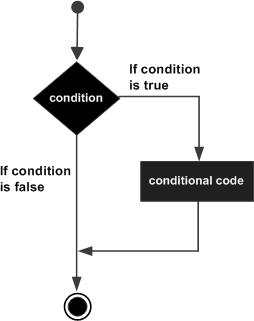
\includegraphics[width=5cm]{c2_perl_if_01.jpg}
  \end{figure}
\end{frame}

\begin{frame}[fragile]
  \frametitle{判断语句 | if | \alert{语法}}
  \vspace{-1em}
\begin{lstlisting}[language=Perl]
# if区块
if ($hour > 22) {
  print "should sleep...\n";
}

# if语句
print "hello" if $guest >= 1;
\end{lstlisting}
\end{frame}

\begin{frame}
  \frametitle{判断语句 | if-else | 逻辑流程}
  \begin{figure}
    \centering
    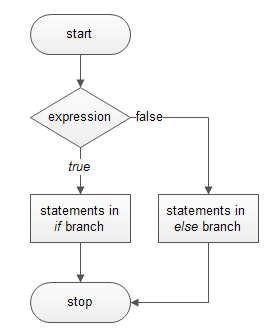
\includegraphics[width=6cm]{c2_perl_if_else_01.png}
    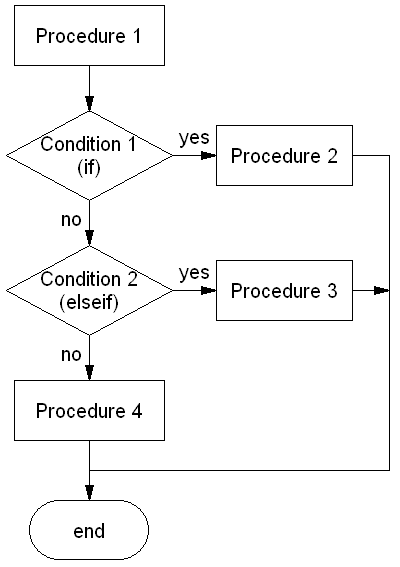
\includegraphics[width=5cm]{c2_perl_elsif_01.png}
  \end{figure}
\end{frame}

\begin{frame}[fragile]
  \frametitle{判断语句 | if-else | \alert{语法}}
  \vspace{-1em}
\begin{lstlisting}[language=Perl]
if ($name eq "Paul") {
  print "Hi Paul\n";
}
elsif ($name eq "Joe") {
  print "Hi Joe\n";
}
elsif ($name eq "Jeremy") {
  print "Hi Jeremy\n";
}
else {
  print "Sorry, have we meet before?";
}
\end{lstlisting}
\end{frame}

\subsection{unless语句}
\begin{frame}
  \frametitle{判断语句 | unless | 逻辑流程}
  \begin{figure}
    \centering
    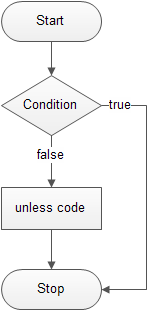
\includegraphics[width=3.5cm]{c2_perl_unless_01.png}
  \end{figure}
\end{frame}

\begin{frame}[fragile]
  \frametitle{判断语句 | unless | \alert{语法}}
\begin{lstlisting}[language=Perl]
# unless区块
unless ($credit > 100) {
  print "You can not graduate!\n";
}

# unless语句
print "eat!\n" unless $food==0;
\end{lstlisting}
\end{frame}

\subsection{given-when语句}
\begin{frame}
  \frametitle{判断语句 | given-when | 逻辑流程}
  \begin{figure}
    \centering
    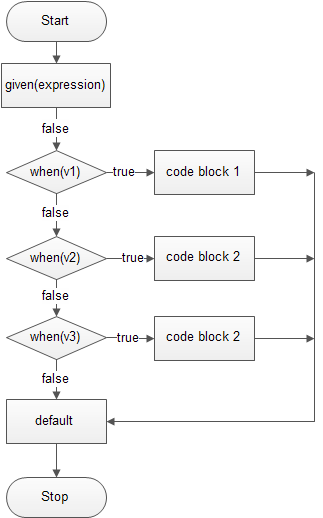
\includegraphics[width=4.5cm]{c2_perl_given_01.png}
  \end{figure}
\end{frame}

\begin{frame}[fragile]
  \frametitle{判断语句 | given-when | 语法}
\begin{lstlisting}[language=Perl]
use 5.010;
given ($foo) {
  say "a" when "a";
  when (/b/) {say "b";}
  default {say "not match";}
}
\end{lstlisting}
\end{frame}

\section{循环语句}
\subsection{foreach语句}
\begin{frame}
  \frametitle{循环语句 | foreach | 逻辑流程}
  \begin{figure}
    \centering
    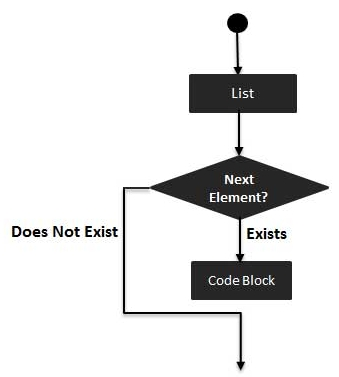
\includegraphics[width=6cm]{c2_perl_foreach_01.jpg}
  \end{figure}
\end{frame}

\begin{frame}[fragile]
  \frametitle{循环语句 | foreach | \alert{语法}}
  \vspace{-1em}
\begin{lstlisting}[language=Perl]
@group = 1..10;

# foreach循环
foreach my $element (@group) {
  print "$element\n";
}

# 等价的for循环
for (@group) {
  print "$_\n";
}
print "$_\n" for @group;
\end{lstlisting}
\end{frame}

\subsection{for语句}
\begin{frame}
  \frametitle{循环语句 | for | 逻辑流程}
  \begin{figure}
    \centering
    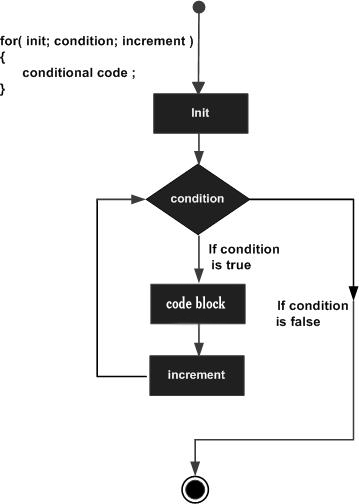
\includegraphics[width=5cm]{c2_perl_for_01.png}
  \end{figure}
\end{frame}

\begin{frame}[fragile]
  \frametitle{循环语句 | for | \alert{语法}}
\begin{lstlisting}[language=Perl]
# 从1数到10
for ($i = 1; $i <= 10; $i++) {
  print "I can count to $i!\n";
}
\end{lstlisting}
\end{frame}

\subsection{while语句}
\begin{frame}
  \frametitle{循环语句 | while | 逻辑流程}
  \begin{figure}
    \centering
    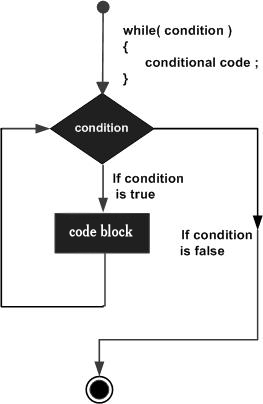
\includegraphics[width=5cm]{c2_perl_while_01.png}
  \end{figure}
\end{frame}

\begin{frame}[fragile]
  \frametitle{循环语句 | while | \alert{语法}}
\begin{lstlisting}[language=Perl]
$i = 0;
while ($i < 10) {
  print "$i\n";
  $i++;
}
\end{lstlisting}
\end{frame}

\begin{frame}
  \frametitle{循环语句 | do-while | 逻辑流程}
  \begin{figure}
    \centering
    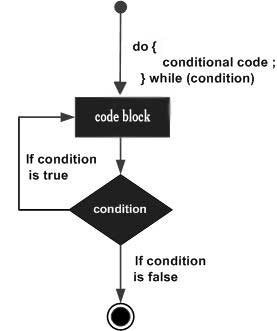
\includegraphics[width=5cm]{c2_perl_do_while_01.jpg}
  \end{figure}
\end{frame}

\begin{frame}[fragile]
  \frametitle{循环语句 | do-while | 语法}
\begin{lstlisting}[language=Perl]
$i = 0;
do {
  print "$i\n";
  $i = $i + 1;
} while ($i < 10);
\end{lstlisting}
\end{frame}

\subsection{until语句}
\begin{frame}
  \frametitle{循环语句 | until | 逻辑流程}
  \begin{figure}
    \centering
    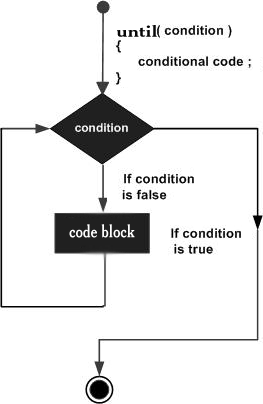
\includegraphics[width=5cm]{c2_perl_until_01.png}
  \end{figure}
\end{frame}

\begin{frame}[fragile]
  \frametitle{循环语句 | until | \alert{语法}}
\begin{lstlisting}[language=Perl]
$i = 0;
until ($i == 10) {
  print "$i\n";
  $i++;
}
\end{lstlisting}
\end{frame}

\begin{frame}
  \frametitle{循环语句 | do-until | 逻辑流程}
  \begin{figure}
    \centering
    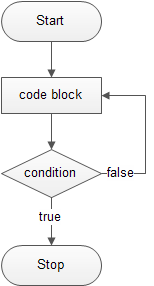
\includegraphics[width=4cm]{c2_perl_do_until_01.png}
  \end{figure}
\end{frame}

\begin{frame}[fragile]
  \frametitle{循环语句 | do-until | 语法}
\begin{lstlisting}[language=Perl]
$i = 0;
do {
  print "$i\n";
  $i++;
} until ($i == 10);
\end{lstlisting}
\end{frame}

\begin{frame}
  \frametitle{循环语句 | 思考}
  \begin{block}{比较}
    \begin{itemize}
      \item 比较while和do-while
      \item 比较until和do-until
    \end{itemize}
  \end{block}
  \pause
  \begin{block}{提示}
    \begin{itemize}
      \item 如果一开始的条件测试就为假,两者的表现有何差异?
    \end{itemize}
  \end{block}
\end{frame}

\section{列表操作}
\begin{frame}
  \frametitle{列表操作 | 简介}
  \begin{block}{\alert{列表操作}}
    基于原来的列表创建一个新的列表:
    \begin{description}
      \item[sort] 将给定列表排序后返回一个新的已排序列表
        \begin{itemize}
          \item 按字母顺序排序 
          \item 按数字顺序排序
          \item 反向排序
          \item 运用sort子程序进行排序
        \end{itemize}
      \item[grep] 筛选列表以寻找符合标准的表项
        \begin{itemize}
          \item 基于原列表筛选大于0的元素建立一个新列表
        \end{itemize}
      \item[map] 将一个列表转换成另一个列表
        \begin{itemize}
          \item 将原列表中的所有元素都乘以2得到新列表
        \end{itemize}
    \end{description}
  \end{block}
\end{frame}

\subsection{sort}
\begin{frame}[fragile]
  \frametitle{列表操作 | sort | \alert{语法}}
\begin{lstlisting}[language=Perl]
sort LIST
sort BLOCK LIST
sort SUBNAME LIST
\end{lstlisting}
  \pause
\begin{lstlisting}[language=Perl]
@passengers = sort @passengers;
@passengers = sort { $a->{age} <=> $b->{age} } @passengers;
@passengers = sort women_and_children_first @passengers;
\end{lstlisting}
\end{frame}

\begin{frame}[fragile]
  \frametitle{列表操作 | sort | \alert{默认排序}}
\begin{lstlisting}[language=Perl]
# sort默认是通过字符串的比较来进行排序的
my @list = sort qw(this is a list);
print "@list";
# a is list this

# sort默认将字符串分成单个字符来进行排序
print join ",", sort qw/1 9 10 99 222/;
# 1,10,222,9,99

# 使用sort代码块将数字按照数字顺序进行排序
print join ",", sort { $a <=> $b } qw /1 9 10 99 222/;
# 1,9,10,99,222
\end{lstlisting}
\end{frame}

\begin{frame}[fragile]
  \frametitle{列表操作 | sort | \alert{反向排序}}
\begin{lstlisting}[language=Perl]
# 执行效率较低:升序排列列表 + 反转列表 = 降序排列列表
my @reversed_names = reverse sort @names;

# 直接反向排序列表
# 反向排序字符串
my @reversed_names = sort { $b cmp $a } @names;
# 降序排序数字
my @descending = sort { $b <=> $a } @numbers;
\end{lstlisting}
\end{frame}

\begin{frame}[fragile]
  \frametitle{列表操作 | sort | 复杂排序}
  \vspace{-1em}
\begin{lstlisting}[language=Perl,basicstyle=\scriptsize\tt]
my @employees = (
    {
        name     => 'Sally Jones',
        years    => 4,
        payscale => 4,
    },
    {
        name     => 'Abby Hoffman',
        years    => 1,
        payscale => 10,
    },
    {
        name     => 'Jack Johnson',
        years    => 4,
        payscale => 5,
    },
    {
        name     => 'Mr. Magnate',
        years    => 12,
        payscale => 1,
    },
);
\end{lstlisting}
\end{frame}

\begin{frame}[fragile]
  \frametitle{列表操作 | sort | 复杂排序}
\begin{lstlisting}[language=Perl]
@employees = 
    sort {
        $b->{years}    <=> $a->{years}
        ||
        $a->{payscale} <=> $b->{payscale}
        ||
        $a->{name}     cmp $b->{name}
    }
    @employees;
\end{lstlisting}
\end{frame}

\begin{frame}[fragile]
  \frametitle{列表操作 | sort | 复杂排序}
  \vspace{-1em}
\begin{lstlisting}[language=Perl]
# 将sort代码块放到子程序中,并用子程序的名称替代sort代码块
sub by_seniority_then_pay_then_name {
    $b->{years}    <=> $a->{years}
    ||
    $a->{payscale} <=> $b->{payscale}
    ||
    $a->{name}     cmp $b->{name}
}

@employees = sort by_seniority_then_pay_then_name @employees;
# 当排序条件很复杂时,使用一个命名的排序子程序:
# 1. 提高代码的可读性
# 2. 便于重复使用
\end{lstlisting}
\end{frame}

\subsection{grep}
\begin{frame}[fragile]
  \frametitle{列表操作 | grep | \alert{语法}}
  \begin{block}{grep:筛选}
    生成一个新的列表,该列表中的所有元素由一个给定列表中所有满足筛选标准的元素组成。 
  \end{block}
  \vspace{-1em}
\begin{lstlisting}[language=Perl]
NEWLIST = grep BLOCK       LIST;
NEWLIST = grep EXPRESSION, LIST;
# 注意逗号的有无!
\end{lstlisting}
\pause
\begin{lstlisting}[language=Perl]
my @greater = grep { $_ > 0 } @numbers;
my @greater = grep   $_ > 0,  @numbers;
my @greater = grep ( $_ > 0,  @numbers );
\end{lstlisting}
\end{frame}

\begin{frame}[fragile]
  \frametitle{列表操作 | grep | 原理}
  \begin{block}{原理}
    在使用grep函数时,通过轮流地把每个元素设置成 \verb|$_| 的方式,可以实现对列表中每个元素的迭代处理。grep函数只返回在BLOCK或EXPRESSION中值为真的那些元素。可以在grep函数中使用任意复杂的表达式。
  \end{block}
  \vspace{-1em}
\begin{lstlisting}[language=Perl]
# 获取回文字符串
my @palindromes = grep { uc eq reverse uc } @words;

# 查找给定列表中以元音字母开头的单词
my @starts_with_vowels = grep { /^[aeiou]/ } @words;
\end{lstlisting}
\end{frame}

\begin{frame}[fragile]
  \frametitle{列表操作 | grep | 组合sort}
\begin{lstlisting}[language=Perl]
my @numbers = ( 13, 3, -2, 7, 270, 19, -3.2, 10.1 );
my @result = sort { $a <=> $b } grep { $_ >= 10 } @numbers;
print join ", ", @result;
# 10.1, 13, 19, 270

# 更加清晰易读
my @result = sort { $a <=> $b }
             grep { $_ >= 10  } @numbers;
\end{lstlisting}
\end{frame}

\subsection{map}
\begin{frame}[fragile]
  \frametitle{列表操作 | map | \alert{语法}}
  \begin{block}{map:变换}
在想要改变整个列表内容时使用map。它逐个对给定列表中的元素进行处理,然后新建一个列表,并将修改后的值返回到新的列表中。 
  \end{block}
  \vspace{-1em}
\begin{lstlisting}[language=Perl]
NEWLIST = map BLOCK       LIST;
NEWLIST = map EXPRESSION, LIST;
# 注意逗号的有无!
\end{lstlisting}
\pause
\begin{lstlisting}[language=Perl]
# 将列表中的每一个字母大写
my @UPPER = map { uc } @words;

# 对列表中的正数求平方根
my @roots = map  { sqrt($_) }
            grep { $_ > 0   } @numbers;
\end{lstlisting}
\end{frame}

\begin{frame}[fragile]
  \frametitle{列表操作 | map | 实例}
  \vspace{-1em}
\begin{lstlisting}[language=Perl]
# 将华氏温度转换为摄氏温度
my %fahrenheit = (
    'absolute zero'    => -459.67,
    'freezing water'   => 32,
    'body temperature' => 98.6,
    'boiling water'    => 212,
);

my %celsius = map 
    { $_ => 5 / 9 * ($fahrenheit{$_} - 32) }
    keys %fahrenheit;
\end{lstlisting}
\end{frame}

\subsection{高效排序}
\begin{frame}[fragile]
  \frametitle{列表操作 | 高效排序}
  \begin{block}{Orcish Maneuver}
\begin{lstlisting}[language=Perl]
keys my %or_cache = @in;
@out = sort {
    ($or_cache{$a} ||= foo($a))
    cmp
    ($or_cache{$b} ||= foo($b))
} @in;
\end{lstlisting}
  \end{block}
  \begin{block}{参考资料}
    \begin{itemize}
      \item \href{https://www.perlmonks.org/?node=130021}{Orcish Maneuver}
      \item \href{https://blog.gtwang.org/perl/orcish-maneuver-perl-sorting/}{Orcish Maneuver:让Perl排序程序加速的方法}
    \end{itemize}
  \end{block}
\end{frame}

\begin{frame}[fragile]
  \frametitle{列表操作 | 高效排序 | foobar}
  \begin{block}{foobar}
foobar是电脑程式领域里的术语,并无实际用途和参考意义。在计算机程序设计与计算机技术的相关文档中,术语foobar是一个常见的无名氏化名,常被作为“伪变量(metasyntactic variable)”使用。\\
\vspace{0.5em}
单词“foobar”或分离的“foo”与“bar”常出现于程序设计的案例中,如同Hello World程序一样,它们常被用于向学习者介绍某种程序语言。\\
\vspace{0.5em}
“foo”、“bar”常被作为函数/方法的名称或变量名。
  \end{block}
\end{frame}

\begin{frame}[fragile]
  \frametitle{列表操作 | 高效排序}
  \begin{block}{\alert{Schwartzian transform}}
\begin{lstlisting}[language=Perl,basicstyle=\small\tt]
# The general form of the Schwartzian Transform:
@sorted = map  { $_->[0] }
          sort { $a->[1] cmp $b->[1] }
          map  { [$_, foo($_)] }
               @unsorted;

# sort the DNA list ("ACGT","A","AC","ACG") according to the sequence length
@sorted_DNA = map  { $_->[0] }
              # 3. extract DNA sequence
              sort { $a->[1] <=> $b->[1] }
              # 2. use numeric comparison
              map  { [$_, length($_)] }
              # 1. calculate the length of the DNA
                   @unsorted_DNA;
\end{lstlisting}
  \end{block}
\end{frame}

\begin{frame}[fragile]
  \frametitle{列表操作 | 高效排序}
  \begin{block}{Schwartzian transform}
\begin{lstlisting}[language=Perl]
# James|007|Spy
# Number 6|6|Ex-spy
# Agent 99|99|Spy with unknown name
# Napoleon Solo|11|Uncle spy
# Unknown|666|Maybe a spy

my @sorted = map  { $_->[0] }
             # 3. undecorate
             sort { $a->[1] <=> $b->[1] }
             # 2. sort
             map  { /\|(\d+)/; [ $_, $1 ] }
             # 1. decorate
                  <>;
\end{lstlisting}
  \end{block}
\end{frame}

\begin{frame}
  \frametitle{列表操作 | 高效排序}
  \begin{block}{参考资料(Schwartzian transform)}
    \begin{itemize}
      \item \href{https://www.wikiwand.com/en/Schwartzian_transform}{Schwartzian transform}
      \item \href{https://www.perl.com/article/the-history-of-the-schwartzian-transform/}{The History of the Schwartzian Transform}
      \item \href{https://en.wikibooks.org/wiki/Algorithm_Implementation/Sorting/Schwartzian_transform}{Algorithm Implementation/Sorting/Schwartzian transform}
      \item \href{https://blog.csdn.net/iSpeller/article/details/48161395}{使用施瓦茨变换(Schwartzian Transform)进行高速排序}
    \end{itemize}
  \end{block}
\end{frame}

\begin{frame}[fragile]
  \frametitle{列表操作 | 高效排序}
  \begin{block}{Guttman-Rosler Transform}
\begin{lstlisting}[language=Perl]
# James|007|Spy
# Number 6|6|Ex-spy
# Agent 99|99|Spy with unknown name
# Napoleon Solo|11|Uncle spy
# Unknown|666|Maybe a spy

my @sorted = map { substr $_, 4 }
    sort
    map {/\|(\d+)/; pack("A4", $1).$_ } <>;
\end{lstlisting}
  \end{block}
  \begin{block}{参考资料}
    \begin{itemize}
      \item \href{http://www.lowlevelmanager.com/2010/10/grt-guttman-rosler-transform.html}{GRT : Guttman Rosler Transform}
      \item \href{https://www.perlmonks.org/?node_id=145659}{Advanced Sorting - GRT - Guttman Rosler Transform}
    \end{itemize}
  \end{block}
\end{frame}

\section{检修脚本}
\begin{frame}[fragile]
  \frametitle{\alert{检修脚本}}
  \vspace{-1em}
\begin{lstlisting}[language=Perl,basicstyle=\small\tt]
# 不洁模式
#!/usr/bin/perl -T

# 打开警告
use warnings;

# 严格模式,语法更加规范
use strcit;

# 开启诊断功能:提供扩展描述来指明具体哪部分程序出了问题,以及关于如何解决这些问题的建议
# 对于初学者非常有用,有经验的程序员通常将其省略
use diagnostics;

# 启用UTF-8编码
use utf8;
\end{lstlisting}
\end{frame}

\begin{frame}[fragile]
  \frametitle{\alert{检修脚本}}
\begin{lstlisting}
# 检查语法
perl -c script.pl

# 格式化脚本
perltidy script.pl

# 调试脚本
perl -d script.pl
\end{lstlisting}
\end{frame}

\begin{frame}
  \frametitle{检修脚本 | 调试}
  \begin{table}
    \centering
    \rowcolors[]{1}{blue!20}{blue!10}
    \begin{tabularx}{0.8\textwidth}{cX}
      \hline
      \rowcolor{blue!50}命令 & 功能\\
      \hline
      s & 仅执行脚本中的一行\\
      n & 按步执行以避免进入子程序\\
      c & 继续运行直至遇到断点\\
      r & 继续运行直至从当前子程序中执行返回命令\\
      v & 显示当前行前后的代码\\
      b & 设置断点\\
      x & 显示变量的值\\
      w & 设置监视表达式\\
      T & 显示栈回溯追踪\\
      L & 列出所有的断点\\
      B & 删除断点\\
      R & 重新启动脚本以便再次测试\\
      q & 退出调试器\\
      \hline
    \end{tabularx}
  \end{table}
\end{frame}

\section{模块}
\begin{frame}
  \frametitle{模块 | Popular Distributions}
  \begin{center}
    \href{https://metacpan.org/favorite/leaderboard}{https://metacpan.org/favorite/leaderboard}
  \begin{figure}
    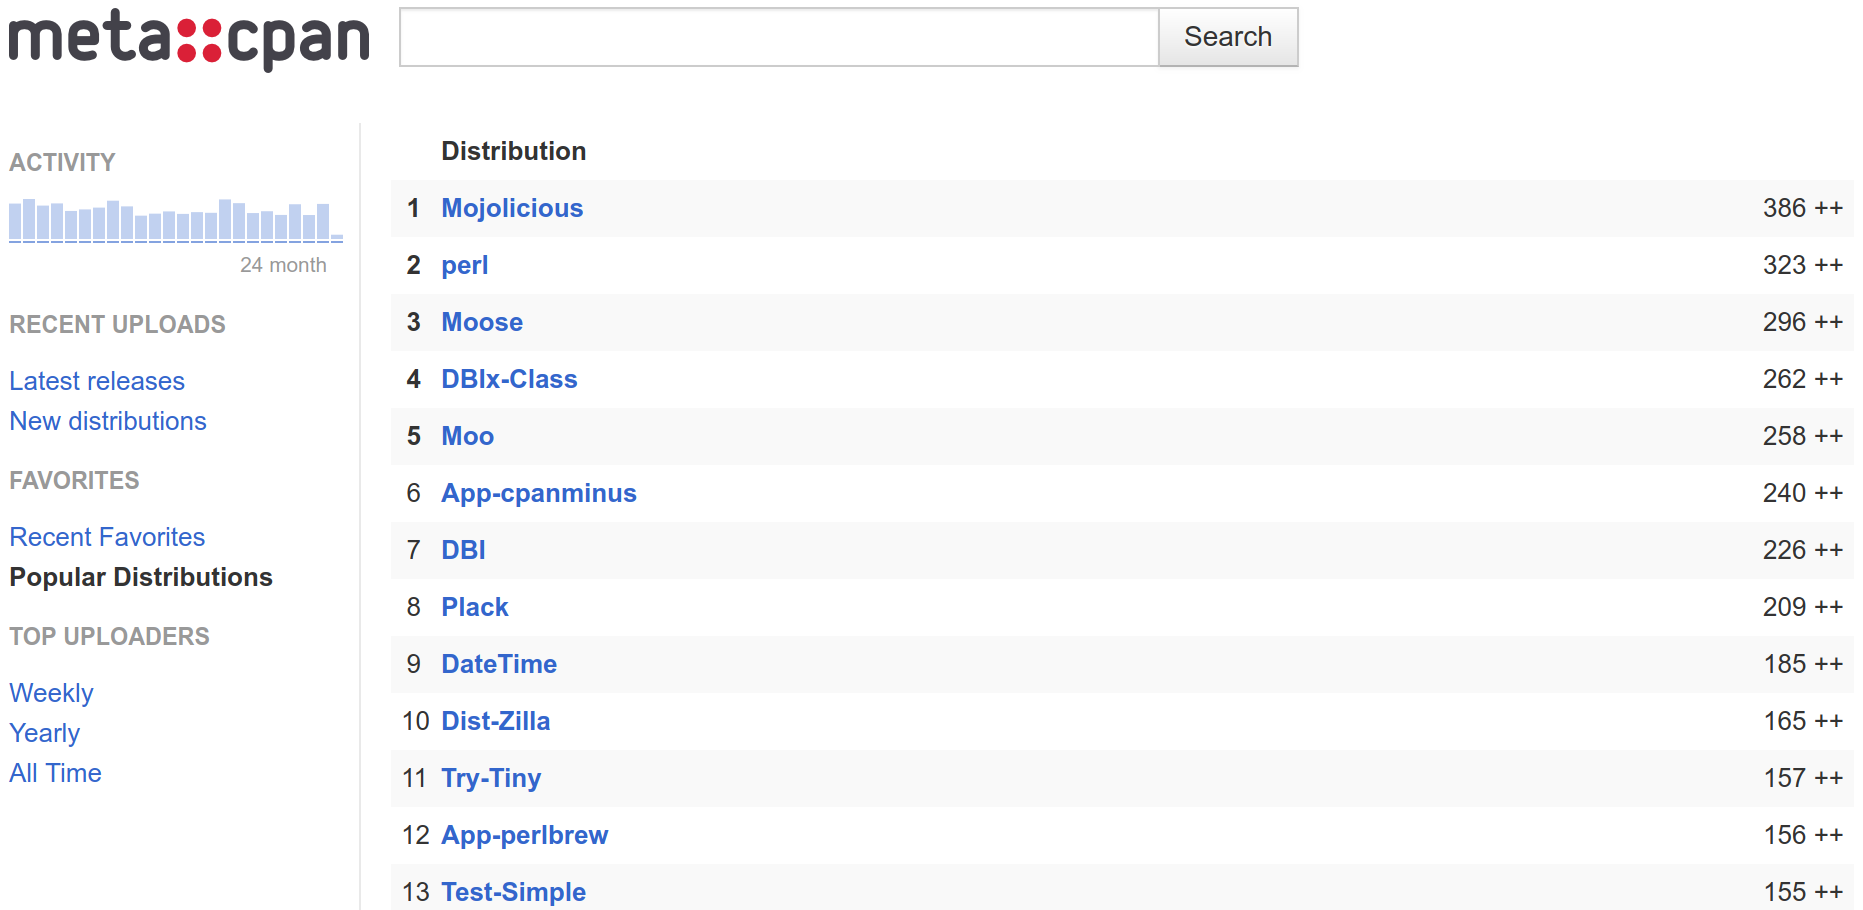
\includegraphics[width=\textwidth]{c2_perl_metacpan_02.png}
  \end{figure}
\end{center}
\end{frame}

\begin{frame}
  \frametitle{模块 | 面向对象}
    \begin{description}
      \item[Moose] A postmodern object system for Perl 5 
      \item[Moo] Minimalist Object Orientation (with Moose compatibility)
      \item[Moops] Moops Object-Oriented Programming Sugar
      \item[Mouse] Moose minus the antlers, a postmodern object system for Perl5
      \item[Role::Tiny] Roles. Like a nouvelle cuisine portion size slice of Moose.
    \end{description}
\end{frame}

\begin{frame}
  \frametitle{模块 | 网站相关}
  {\footnotesize
    \begin{description}
      \item[Mojolicious] Real-time web framework 
      \item[Dancer] lightweight yet powerful web application framework 
      \item[Dancer2] Lightweight yet powerful web application framework 
      \item[Catalyst] The Elegant MVC Web Application Framework 
      \item[PSGI] Perl Web Server Gateway Interface Specification
      \item[Mojo::Pg] Mojolicious ♥ PostgreSQL
      % \item[Mojo::Pg] Mojolicious $\varheartsuit$ PostgreSQL
      \item[LWP] The World-Wide Web library for Perl 
      \item[Plack] Perl Superglue for Web frameworks and Web Servers (PSGI toolkit) 
      \item[Starman] High-performance preforking PSGI/Plack web server
      \item[Template] Front-end module to the Template Toolkit
      \item[Text::Xslate] Scalable template engine for Perl5
      \item[HTTP::Tiny] A small, simple, correct HTTP/1.1 client
      \item[WWW::Mechanize] Handy web browsing in a Perl object
      \item[HTML::FormHandler] HTML forms using Moose
      \item[URI] Uniform Resource Identifiers (absolute and relative)
      \item[HTTP::Message] HTTP style message (base class)
    \end{description}
}
\end{frame}

\begin{frame}[fragile]
  \frametitle{模块 | 实用工具}
    \begin{description}
      \item[App::perlbrew] Manage perl installations in your \verb|$HOME| 
      \item[App::cpanminus] get, unpack, build and install modules from CPAN
      \item[ack] grep-like text finder
      \item[Perl::Tidy] Parses and beautifies perl source
      \item[App::FatPacker] pack your dependencies onto your script file
      \item[Devel::NYTProf] Powerful fast feature-rich Perl source code profiler
      \item[Carton] Perl module dependency manager (aka Bundler for Perl)
      \item[Devel::REPL] A modern perl interactive shell
      \item[Reply] read, eval, print, loop, yay!
      \item[Ubic] polymorphic service manager
      \item[Rex] Remote Execution
      \item[\alert{Smart::Comments}] Comments that do more than just sit there
      \item[\alert{Benchmark}] benchmark running times of Perl code
    \end{description}
\end{frame}

\begin{frame}
  \frametitle{模块 | Utils}
    \begin{description}
      \item[Scalar::Util] A selection of general-utility scalar subroutines
      \item[\alert{List::Util}] A selection of general-utility list subroutines
      \item[List::MoreUtils] Provide the stuff missing in List::Util
      \item[List::SomeUtils] Provide the stuff missing in List::Util
      \item[List::UtilsBy] higher-order list utility functions
      \item[List::AllUtils] Combines List::Util, List::SomeUtils and List::UtilsBy in one bite-sized package
      \item[Hash::Util] A selection of general-utility hash subroutines
      \item[Sub::Util] A selection of utility subroutines for subs and CODE references
    \end{description}
\end{frame}

\begin{frame}
  \frametitle{模块 | 脚本编写}
    \begin{description}
      \item[Modern::Perl] enable all of the features of Modern Perl with one import
      \item[Cwd] get pathname of current working directory
      \item[File::Spec] portably perform operations on file names
      \item[FindBin] Locate directory of original perl script
      \item[Path::Tiny] File path utility
      \item[Path::Class] Cross-platform path specification manipulation
      \item[local::lib] create and use a local lib/ for perl modules with PERL5LIB
      \item[Type::Tiny] tiny, yet Moo(se)-compatible type constraint
      \item[Term::ANSIColor] Color screen output using ANSI escape sequences
      \item[AnyEvent] the DBI of event loop programming
      \item[File::Temp] return name and handle of a temporary file safely
      \item[Log::Log4perl] Log4j implementation for Perl
      \item[Log::Any] Bringing loggers and listeners together
      \item[IO] load various IO modules
      \item[Sereal] Fast, compact, powerful binary (de-)serialization
    \end{description}
\end{frame}

\begin{frame}[fragile]
  \frametitle{模块 | 开发测试}
    \begin{description}
      \item[Perl::Critic] Critique Perl source code for best-practices
      \item[Encode] character encodings in Perl
      \item[Regexp::Debugger] Visually debug regexes in-place
      \item[autodie] Replace functions with ones that succeed or die with lexical scope
      \item[Carp] alternative warn and die for modules
      \item[Devel::Cover] Code coverage metrics for Perl
      \item[Devel::hdb] Perl debugger as a web page and REST service
      \item[Test::Harness] Run Perl standard test scripts with statistics
      \item[Test::Simple] Basic utilities for writing tests
      \item[Test::Deep] - Extremely flexible deep comparison
      \item[Try::Tiny] minimal try/catch with proper preservation of \verb|$@| 
      \item[Capture::Tiny] Capture STDOUT and STDERR from Perl, XS or external programs
      \item[PPI] Parse, Analyze and Manipulate Perl (without perl)
    \end{description}
\end{frame}

\begin{frame}
  \frametitle{模块 | 数据格式}
  {\footnotesize
    \begin{description}
      \item[DBIx::Class] Extensible and flexible object <-> relational mapper
      \item[DBI] Database independent interface for Perl 
      \item[DBIx::Class::Schema::Loader] Create a DBIx::Class::Schema based on a database
      \item[MongoDB] Official MongoDB Driver for Perl
      \item[Mango] Pure-Perl non-blocking I/O MongoDB driver
      \item[JSON] JSON (JavaScript Object Notation) encoder/decoder
      \item[DateTime] A date and time object for Perl 
      \item[Time::Moment] Represents a date and time of day with an offset from UTC
      \item[Data::Printer] colored pretty-print of Perl data structures and objects
      \item[\alert{Data::Dumper}] stringified perl data structures, suitable for both printing and eval
      \item[Imager] Perl extension for Generating 24 bit Images
      \item[Text::CSV] comma-separated values manipulator (using XS or PurePerl)
      \item[XML::LibXML] Perl Binding for libxml2
      \item[SQL::Abstract] Generate SQL from Perl data structures
      %\item[YAML] YAML Ain't Markup Language™
      \item[YAML] YAML Ain't Markup Language\texttrademark
      \item[XML::Twig] A perl module for processing huge XML documents in tree mode
      \item[Redis] Perl binding for Redis database
    \end{description}
}
\end{frame}

\begin{frame}
  \frametitle{模块 | Others}
    \begin{description}
      \item[\alert{Getopt::Long}] Extended processing of command line options
      \item[File::Slurp] Simple and Efficient Reading/Writing/Modifying of Complete Files
      \item[IO::All] IO::All to Larry Wall!
      \item[\alert{Parallel::ForkManager}] A simple parallel processing fork manager
      \item[MCE] Many-Core Engine for Perl providing parallel processing capabilities
      \item[POE] portable multitasking and networking framework for any event loop
      \item[Coro] the only real threads in perl
      \item[Dist::Zilla] distribution builder; installer not included
      \item[Time::HiRes] High resolution alarm, sleep, gettimeofday, interval timers
      \item[CHI] Unified cache handling interface
      \item[Minion] Job queue
      \item[Daemon::Control]Create init scripts in Perl
    \end{description}
\end{frame}

\section{回顾与总结}
\subsection{总结}
\begin{frame}
  \frametitle{Perl语言入门 | 总结}
  \begin{block}{知识点}
    \begin{itemize}
      \item Perl语言简介:基本知识,中心思想,优缺点,语法结构
      \item 变量:标量,数组,散列,内置变量
      \item 操作符:数字、字符串、逻辑、文件测试、匹配操作符
      \item 基本函数:print, chomp, join, split, open, close, my
      \item 判断语句:if, unless, if-else, given-when
      \item 循环语句:foreach, for, while, until
      \item 列表操作:sort, grep, map
      \item 检修脚本:检查语法,格式化脚本,调试脚本
    \end{itemize}
  \end{block}
  \begin{block}{技能}
    \begin{itemize}
      \item 掌握Perl语言的基本语法
      \item 使用Perl编写简单的应用脚本
    \end{itemize}
  \end{block}
\end{frame}

\subsection{思考题}
\begin{frame}
  \frametitle{Perl语言入门 | 思考题}
  \begin{enumerate}
    \item Perl语言的中心思想是什么?
    \item Perl中的变量主要有哪三大类?
    \item 列举Perl中的各种操作符。
    \item chomp, join, split的作用是什么?
    \item 在Perl中如何和文件进行交互?
    \item Perl中的判断语句有哪些,语法是怎样的?
    \item Perl中的循环语句有哪些,语法是怎样的?
    \item 列举Perl中进行列表操作的函数。
    \item 如何调试Perl脚本?
  \end{enumerate}
\end{frame}

\begin{frame}
  \frametitle{下节预告}
  \begin{itemize}
    \item 在面对问题的时候,你是如何构思解决策略的?
    \item 在编程中,你是怎样保存和备份程序的?
    \item 你是如何一步一步从零开始写出一个可用程序的?
  \end{itemize}
\end{frame}


\input{snippet/class_tail}
